%!TEX root = project.tex

\chapter*{About this project}
\paragraph{Abstract}
Mobile apps are becoming more prevalent in our everyday lives, enabling people to complete a variety of tasks using their mobile devices. Despite promoting innovation, the smartphone market's rapid growth has resulted in some divergence of mobile platforms.

When we want to build mobile applications for multiple platforms, having multiple mobile operating systems with different programming languages and resources can be a challenge. In general, rewriting applications for each platform makes no sense financially or temporally.

As a consequence, a solution that can create cross-platform apps without sacrificing quality will minimize time to market and expand the number of potential users. Fortunately, some work has been done in recent years to address this problem, including the use of web technology, cross-platform tools, and frameworks.

This dissertation proposes the use of cross-platform framework flutter to build cross-platform apps. It Cover's an  Android app build using flutter. These types of frameworks suggest defining platform-independent models to characterize mobile applications and automatically generating source code for multiple platforms using these models.
This dissertation introduces the Dart language and Flutter framework assesses it and discusses its main challenges and benefits in the context of developing mobile applications.

\paragraph{Authors}
Muhammad Noman Junaid and Muhammad Luqman are 4th-year Students of B.SC (Hons) in Computing in Software Development in GMIT.



\chapter{Introduction}
\section{The Idea}
Our project is an Android photo and sharing social networking application named City Social. The general concept of our application was to create a social network app that mirrors Instagram But we changed our ideal later and decided to built something different.So our app differs in a way that it shows social feed of all users on the app network instead of only followed users like in other apps.

According to \cite{COVID19-SocialMediaUsage:online} Everyone these days especially during this Covid-19 pandemic spend most of their time in social activities on social networking apps such as Facebook, snap-chat, Instagram, etc and their usage is around 72\%  So the Specific goal of this project was to learn how to create one of these apps and to learn how these apps work back-end.

And one of the most important goals of this project was learning something new so we decided to build an photo sharing social network app using the new technologies which were not known to us at that time such as Cross-platform Framework Flutter, Dart Language, and Firebase.
\section{Solution Formation}
Our app is like for a city in which all people can see and interact with posts from same city users that's why we named our app city social.Our app features signing in and sign up using Email and password, posting photos along with captions,liking posts of other users and also commenting on posts.We have also implemented group chat feature in which users can create a group and chat with each other.we have profile page which is something similar to Instagram in which number of followers, number of following users and number of posts is displayed.There is a recently added section below them in which all posts of following users is displayed ordered by timestamp means most recent first.

A focus that we made on our Application is integrating different technologies mentioned above. Using these technologies made certain aspects of our application easier to implement.

\subsection{Flutter}

Flutter UI toolkit by Google for building fast creative applications for mobile, web, and desktop from a single codebase. it’s a cross-platform tool for creating Android and iOS apps from a single code base by using a modern, reactive framework \cite{WhatisFl74:online}. Dart is a simple programming language that is used to created flutter applications The core idea of Flatter revolves around widgets. The entire user interface consists of a combination of different widgets, each widget defines structural elements (such as buttons or menus), style elements (such as fonts or color schemes) and design aspects, and so on.
\subsection{Firebase}
Firebase is another feature-rich technology we use. It has many products, such as Cloud Firestore, which uses a NoSQL database hosted in the cloud to store and synchronize data between users and devices around the world. Authentication via email, password, and external providers (such as GitHub, Google, Facebook, and Twitter). A real-time database, an efficient and low-latency solution, is suitable for mobile applications that require real-time status synchronization between clients. 
\subsection{Cloud FireStore}
Cloud Firestore, also known as Google Firestore, is part of the Google Firebase platform. This is a cloud NoSQL database server that does an excellent job of storing and synchronizing data. In fact, web and mobile applications can directly interact with Firestore when in use. Native SDK. Firestore is a high-performance database that supports auto-scaling. It is also very easy to use and very reliable.

\subsection{Dart}
Dart was developed to make it as convenient and fast as possible for developers. Therefore, it contains many extensive integrated tools such as its own package manager, various compilers/compilers, parsers, and formatters. In addition, the virtual dart machine and timely compilation make code changes immediately executable. In the production environment, the code can be compiled locally, so no special environment is required to run. During web development, the dart will be played. In terms of syntax, dart languages such as JavaScript, Java, and C++ are very similar, so it takes several hours to learn dart knowledge in one of these languages.

\section{Project Plan}
From our initial supervisor meetings, we developed a simple outline of the work to be concluded within the time frame but after the review from our supervisor and the panel review in May 2021 we changed our app idea a little and decided to recreate the project so in June we started recreating the App. The outline below spans from October 2020 to July 2021.
\begin{itemize}
\item October to April - Initial Research, decided technologies, created starter project added splashscreen, authentication, navigation pages, header and widgets, implemented database, upload functionality, profile page edit and timeline functionality and like/unlike functionality, comments functionality .
\item May - Work on dissertation and after app review as discussed above we changed our app idea so started research about different UI \& features to include in our new app that will be  different from the previous one developed.
\item June - Started creating the app again from scratch. Created a new GitHub Repository and a new flutter project.Added Authentication and firebase services in the project.Added signing up with Email and signout functionality.Added firebase operations for fetching user data and implemented the use of picture as a user display picture, stored user data to firebase and fetch it, worked on timeline home page , profile page and chat, created a bottom navigation bar, work on Dissertation.
\item July - Fixed a sign up bug \#1, added more information on profile page, stored the upload image with caption to firebase and fixed the upload image bug \#2, post functions(like,comments) added, Fixed bug of overflown widget \#3,implemented timestamp feature,worked on homepage UI, work on Dissertation.
\item August - implemented Delete post function, fixed \#5 bug of overflown widget, follow feature added, fetched profile data,implemented chat function,Made test cases and tested the app, Fixed all other bugs mentioned on github and worked on Dissertation and Created a screen cast of the App.
\end{itemize}

\subsection{Project Task}
As we both were new to all three technologies so we mostly did most of the work together so as we both we working as well so we would meet at a same place after work and then work together on the project for 4 to 5 hours.We thought that instead one person works on front end and one on back end we would work together so that both of us knows how the both aspects work.Because if we did that separately then one would know backend or frontend only.So we learned together and the way we did it was sometimes "Luqman" would code and "Noman" assist him and sometimes "noman" would code and "Luqman" assisted him.

\subsubsection{Tasks coded By Luqman}
\begin{itemize}
    \item Created Github repository.
    \item Created new flutter project.
    \item Added Authentication and its methods.
    \item Added Sign-out functionality
    \item Fixed Bug no 1, no 2, no 3, no 6, no 9, no 12, no 13, no 14
    \item Time Stamp Feature
    \item Follow Functionality
    \item Group Messages Functionality
    \item Test Plan / Cases
    \item Performance Testing
    \item Dissertation
    
\end{itemize}

\subsubsection{Tasks coded By Noman}
\begin{itemize}
    \item Sign-in \& Sign-up Functionality
    \item HomePage UI.
    \item Bottom Navigation Bar.
    \item Profile Page UI
    \item Likes \& Comments Functionality
    \item Posts display on Timeline
    \item Delete post Functionality
    \item Fixed Bug no 5, no 7, no 8, no 10, no 11
    \item Displaying posts on profile page
    \item Chatroom UI and Create Chatroom Functionality
    \item Testing
    \item Dissertation
\end{itemize}

\section{Objectives for Project}
The main objectives of this project are to learn new technologies such as flutter framework, dart language, and Firebase integration.

All features of our app were our objectives and some Objectives and Requirements are:
\begin{itemize}
\item Learn Flutter Framework, Dart and Firebase (requirement)
\item Create Fast responsive application (requirement)
\item Create a Scalable and Re-Usable application (requirement)
\item Implement planned features.
\end{itemize}

\section{Chapter Descriptions}
\subsubsection{Methodology}
In this chapter, we will discuss the methodology that we used in the development of our project and how it has aided us in the development process. The methodology we used was agile, it helped us to increment development on a weekly basis and to keep workflow moving consistently. Also, it will mention the different development tools we used to collaborate and develop the project and also the way in which we stayed in contact to deliver the project

\subsubsection{Technology Review}
Above we gave a small introduction of the technologies that we used but
In this chapter, we will discuss the different technologies we used for the development of our project in detail, and we will explain why we choose these technologies for our project. We will be describing how these different technologies played a role in the development of the project and how they worked together.

\subsubsection{System Design} 
In this section of the documentation, we will discuss the architecture of the project, we also will be discussing the research that went into the construction of the project. We will be discussing how all the elements interact with one another. Also, there will be screenshots of UI components.

\subsubsection{System Evaluation}
In this section, we will discuss how we tested out our project and analyzed its performance, and see if we can find any limitations and evaluate our project against the objectives we set out. We will reflect on the various problems we came across and the solutions that came with them.

\subsubsection{Conclusion}
In this chapter, we will discuss the conclusion of our project, we will discuss the outcomes of the project, and also the knowledge we have gained from doing the project and further scope or opportunities.

\section{GitHub Repository}
The URL of Our GitHub Repository is \url{https://github.com/LuqmanFarooq/Final-Year-Project-And-Dissertation}.
\subsection{Source Code Of App}
It contains the source code of the Application developed on the root directory of the repo.
\subsection{Testing of App}
There is a folder named \textbf{1- Testing of App} which contains all material related to the testing of our app.
\subsection{Apk Installation File}
There is a folder called \textbf{2-APK FILE} that contains the apk file of the app which can be transfered to any andriod phone and can be installed.
\subsection{Images}
There is an \textbf{3-Images Used} folder in the root that contains the images used in Project Dissertation.
\subsection{Dissertation}
There is an \textbf{4-Dissertation} folder in the root of repository which contains the dissertation files.
\subsection{5-Screencast Demo}
There is an \textbf{5-Screencast Demo} folder in the root of Repository which contains the video Demonstration of the APP.
\subsection{Readme}
There is a ReadMe File Which Gives Overview of the Application its features and instructions of using the Application.

\begin{figure}[!htb]
    \centering
    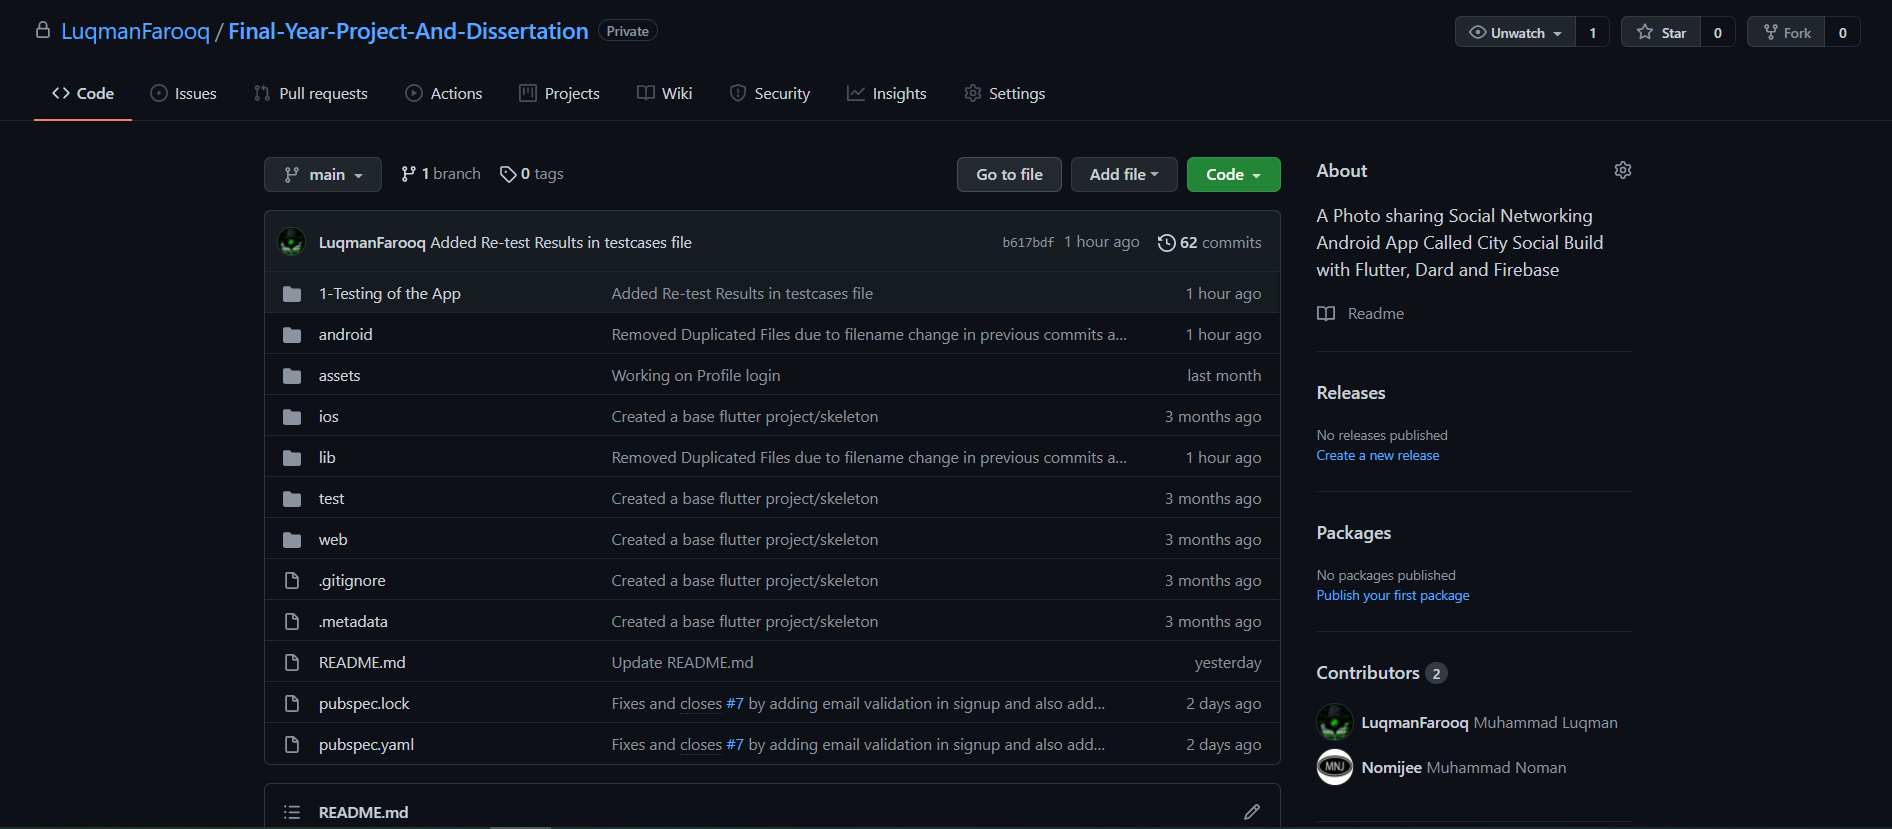
\includegraphics[scale=0.35]{img/github.PNG}
    \caption{GitHub Repository of the Project}
    \label{fig:GitHub Repository of the Project}
\end{figure}
\chapter{Methodology}
This chapter covers the various methodologies that were implemented in this project, describes the methodology that was used and how we implemented it, and also talks about how the development of the project progressed in the end. At the end of this chapter, the reader should be able to have a good impression of the scale of the project and the necessary steps that were taken throughout the project. For our final year project, we both wanted to use a constant design process to which changes and issues could be kept accounted for and so that we would be able to deal with them when they happened in an easy and dynamic way. As a result, we decided to use the Agile method would be the best fit for us as we had both had experience and knowledge of it from our previous years from the course. An Agile methodology is a certain approach to the management of a project which is greatly suited to us doing any project in Software Development. Using this method will help us to come up against any problems or difficulties such as code errors, changing the format of the project so as to suit the client's demands, etc. Agile uses work sequences that are called ‘Sprints’ which is a course of time that’s designated for certain stages in the development of a project. When creating a project, time is an important factor especially when one does Software Development so the idea of using Sprints is very important.

\section{Project Management}
\begin{figure}[!htb]
    \centering
    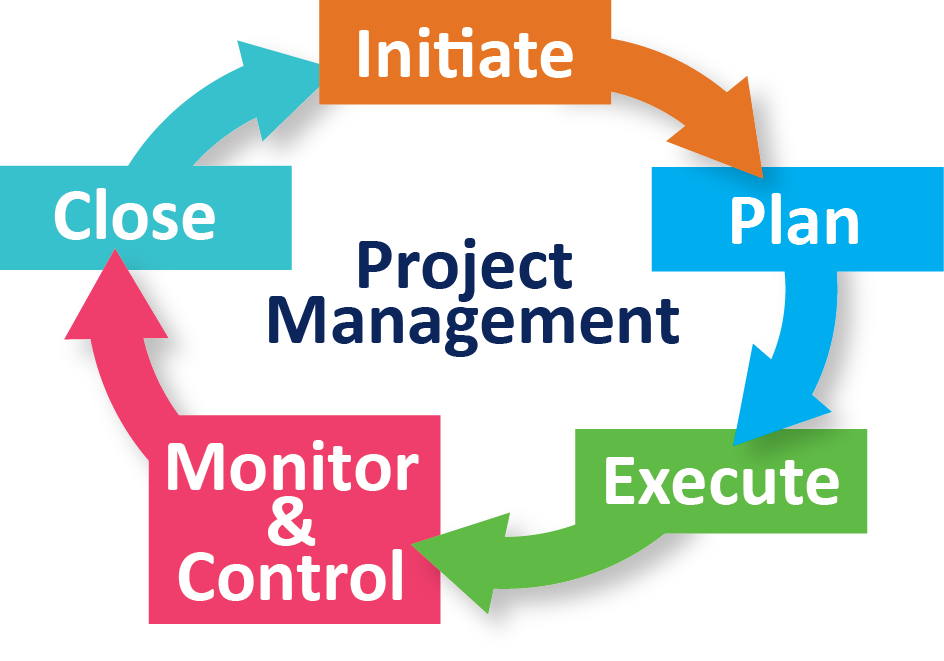
\includegraphics[scale=0.45]{img/Project Management Cycle Framework V2.png}
    \caption{Project Management Cycle Framework}
    \label{fig:Project Management Cycle Framework}
\end{figure}
Project Management is a key element of any task to ensure that the project
is laid out correctly and each component party is complete at a given date.
Because this project is a Group project we used the GitHub Kanban board to first pick features that we may want to implement and then broke them down into
separate cards that we could work on individually. This helped break down tasks
which helped in development. Project management also includes supervisor meetings and Source Control such as GitHub and Overleaf.

\subsection{Agile}
This project used Agile project management methodologies \cite{WhatisAg86:online}. An iterative approach was taken. This meant that each week we had certain tasks laid out to
be completed like a feature for the app. we also had short weekly meetings with our supervisor where we would update him,
and asks for advice on our dissertation, app, and discussed issues that we came across while developing the app, etc.

\subsubsection{Planning and Development}
During the meeting and planning phase, the milestones and objectives for the
project were identified and broken down into simpler, and more manageable tasks. The tasks are were then grouped into sprints or iterations lasting one
to three weeks depending on the task. These are the tasks which mostly completed before each meeting with our supervisor. With each meeting, we had a task somewhat completed and we could then know the following task which we could
talk with our supervisor about beforehand. So each weekly meeting with the
supervisor started a sprint and the aim was to complete most of that sprint
before the next meeting. The plans for the project and the sprints are taken
from the User stories we created on the Kanban project and Design document.
Through this iteration, we convert the plans into working code.
\subsubsection{Design Phase}
Throughout the agile development life cycle, design is a step in every iteration/sprint. The design is gradually built on. The design is never defined at the beginning of the project. The gradual evolution of the design enables taking advantage of new technologies that come on stream as well as meeting any
new requirements brought forward by clients. The user experience is key when
designing a project/application. Every design must be user-friendly \cite{AgileSof90:online}.

The type of end-user of the item must be considered when designing. This comes to play in Flutter development often as there are many different tools in development to create different features. we need to test them to know what's best for the end product e.g there are loads of icons of the came category built in a flutter that we can use have used.
\subsubsection{Testing}
Testing was carried out continuously with Visual Studio Code Emulator. Visual Studio Code has a huge amount of features the Emulator can test
a massive array of devices. So testing for this application was a continuous
process throughout every build.

we will discuss testing \& Performance more in detail in System Evaluation chapter.

\subsubsection{Version Control}
Version control is the practice of tracking and managing code changes. The source code management (SCM) system provides a history of code development execution and helps resolve conflicts when merging contributions from multiple sources. For this
project, we choose Git with GitHub as our Version Control System to track our changes, log errors, and work effectively using our Agile methodology. Git is an open-source and free version control system that allows small or large projects to be stored and accessed efficiently. Features include commits, branching, staging, and workflows. GitHub allows a project to be stored remotely and for multiple people to work together seamlessly \cite{GitHub:online}.

we didn't make our own branches we just committed to the one and only master branch because as discussed in the introduction chapter above that we both worked together. But sometimes we worked simultaneously as well such as during august when the deadline of the project was near we worked at the same time on the project to increase our productivity. We also used inbuilt features on GitHub such as issue tracking. if an issue occurred or a bug was found during testing, we would make a GitHub issue, and log all our commits using the issue id. This would track our progress in fixing it and help us keep an account of the work undertaken.

\chapter{Technology Review}
This chapter discusses the different technologies used throughout the project. It discusses the advantages and disadvantages of each technology and why certain technologies were used over others. It also discusses hybrid applications compared to native applications, advantages, disadvantages, uses at different business structures, and other topics.

\section{Overview}
This Project is a Cross-platform application built with Flutter \& Dart in Visual Studio Code. Firebase is used for the database, authentication, and CRUD functionality of the app.
The following topics are discussed in detail:

\begin{itemize}
\item Flutter
\item Dart
\item Firebase
\item Apptim
\end{itemize}

\section{Flutter}
\begin{figure}[!htb]
    \centering
    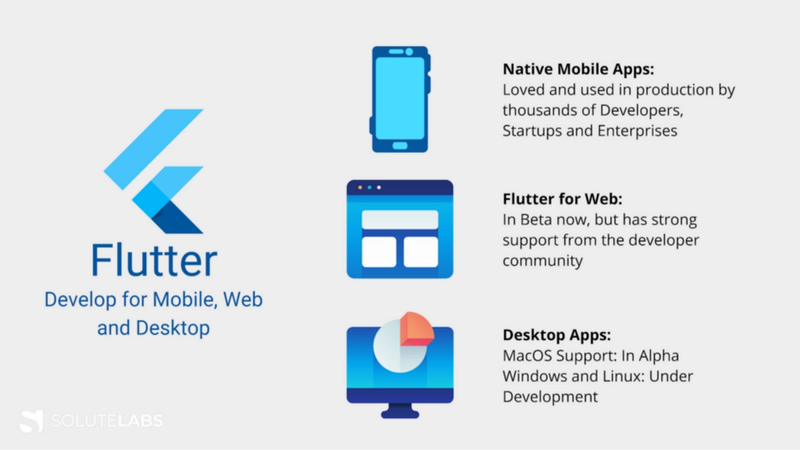
\includegraphics[scale=0.15]{img/Flutter.png}
    \caption{Flutter}
    \label{fig:Flutter}
\end{figure}
Flutter is Google's cross-platform framework that can build beautiful applications for mobile, web, and desktop using a single code base  \cite{FlutterGoogle:online}. The Reason we choose flutter framework is because we wanted to create a cross platform app but for cross platform app development there are other good options as well such as React, xamarin and Ionic but as we used xamarin in our 2nd year and used React and Ionic in our 3rd year so we wanted to try a new competitor so after research we decided to go for flutter.
\subsection{how it works}
\subsubsection{Widgets}
The use of widgets is at the heart of Flutter. Developers can construct a comprehensive user interface by integrating multiple widgets. A structural element (such as a button or menu) and a style element (font or color scheme) are defined by each of these widgets. Aspects of design (for example, interior decoration) and many more.

Flutter also provides responsive views for developers. In order to avoid performance problems when using a compiled programming language to connect to JavaScript, Flutter uses Dart. Pre-compile Dump (AOT) into native code for multiple platforms.

According to \cite{WhatisFlutter-Benefits:online} Flutter is the only mobile SDK that provides reactive views without a JavaScript bridge. This is why so many mobile developers test it in their projects.

Flutter comes with many powerful basic widgets, the following are commonly used:

\subsubsection{Text}
The Text widget helps you to create a run of styled textual content inside your application \cite{widgetsFlutterDev:online}.
\subsubsection{Row, Column}
With flex widgets, we can create bendy layouts in each of the horizontal (row) and vertical (column) directions. The layout of those items is primarily based totally on the web’s flexbox format model \cite{widgetsFlutterDev:online}.
\subsubsection{Stack}
you can stack widgets in the order in which they are drawn. You can then use the widgets located on the children of the stack to position them relative to the top, right, bottom, or left side of the stack. The stack is based on an absolute design model for web page positioning \cite{widgetsFlutterDev:online}.
\subsubsection{Container}
we can use container widgets to create rectangular shapes and can decorate the container with BoxDecoration elements (such as background, frame, or shadow). The container can also have margins, padding, and limits appropriate to its size. You can use an array to convert the container into a 3D space \cite{widgetsFlutterDev:online}.

\subsection{Benefits of Flutter}
Flutter is one of the most advanced mobile applications available today. With the advantage of the development team, it is a strong competitor and will become the preferred mobile technology in the near future. \cite{WhatisFlutter-Benefits:online}. Following are the Advantages of Flutter:
\subsubsection{Saves time and money}
Flutter is a cross-platform development environment. This means that software developers can use the same code base to create iOS and Android apps. Cross-platform development is the most effective way to save time and money throughout the development process.
\subsubsection{Excellent performance}
Flutter provides exceptional results for two reasons. First, it employs Dart, which compiles into native code. Second, since Flutter has its own widgets, there is no need to use OEM ones. As a consequence, contact between the app and the network is reduced. These two Flutter features ensure faster app startup times and fewer overall performance problems.
\subsubsection{Quick development thanks to hot reload}
With its hot reinstallation feature, Flutter is becoming more and more popular among mobile developers. Hot reloading allows you to view code improvements in the simulator, simulator, and hardware in real-time. In less than a second, the code changed. At the same time, the software is up and running, and developers don't have to waste time restarting it. It’s now easier to build user interfaces, add new features, and fix bugs. When an application encounters an error, you can usually fix it and continue using the application as if the error had never occurred. If you need to restart the application, you can ensure that it will be completed quickly, speeding up the development process.
\subsubsection{Compatibility}
Another advantage of Flutter is that it has its own widgets, which means fewer usability issues. Developers will encounter fewer problems with operating system versions and will spend less time testing software on earlier versions of operating systems. Ensure that its software can be used on future operating system models. When a new version of Android or iOS is released, the Flutter widgets need to be changed (because the tool does not use native platform widgets). How to update Flutter's widgets Since Google uses Flutter on a large scale internally, the Flutter team is eager to update its widget set to be as similar as possible to platform widgets. Flutter widgets can also be customized and changed by anyone. With an old version of the operating system, your application may even use new widgets!
\subsubsection{Open-source}
Flutter is an open-source application, surrounded by a group of active developers who provide help, provide complete tool documentation and create useful tools. Dart is completely free.

\subsection{Example Apps Developed with Flutter}
\begin{enumerate}
    \item Google Ads
    \item AppTree
    \item Reflectly
    \item inLapp Coffee
    \item SSHButtons
\end{enumerate}

\section{Dart}
Dart is a client-oriented programming language that can be used to build fast applications on any platform. The purpose is to provide the most powerful programming language for cross-platform development and to provide a common runtime platform for application frameworks. Customer development should give priority to the development of various build targets (Web, mobile, and desktop)  and high-quality manufacturing experience \cite{DartDev5:online}.

As Flutter only supports Dart language so we had to use Dart.

\subsection{The Language}
The Dart programming language is type-safe and uses static type checking to ensure that the value of a variable always matches the static type of the variable. This is commonly referred to as "tone dialing". Although the type is required, type annotations are optional due to type inference. The dart typing scheme also has multiple uses, allowing dynamic typing to be combined with runtime checking, which is very useful when experimenting or when a lot of moving code is required. \cite{DartDev5:online}.

\subsubsection{Sample Program}
Every app has a main() function. To display text on the console, you can use the top-level print() function \cite{LanguageSampleDart:online}:
\begin{minted}{Dart}
void main() {
  print('Hello, World!');
}
\end{minted}

\subsection{Strengths \& Weaknesses of Dart}
Dart has a lot of benefits, but it also has some drawbacks:
\subsubsection{Advantages}
Dart is an open-source programming language that anyone can use for free. Google is the creator of the dart. Given that it is funded by such a large company, the language has a bright future. The dart syntax makes it easy for programmers to learn. Many complex syntactic principles of other languages have been skillfully simplified and revised by their creators. Anyone who has used C\# before can easily learn dart. The programming language was created with the Internet in mind. .Dart can be easily converted directly to JavaScript, so it can be used in modern smartphone browsers and desktop computers. All you need is a simple text editor to program in this language. However, this requires a deeper understanding of programming languages. Special editors such as Android Studio (Google) and Visual Studio Code make work easier (Microsoft).

some big advantages are below:
\subsubsection{Preemptive Scheduling}
There are many programming languages in the market, such as Java, Kotlin, Objective-C, and Swift, which tend to switch between different threads, such as B. Multiple threads run at the same time. Here, a certain period of time is allocated to each thread. In the case that the process is overwritten, the context switch will take care of that specific thread to execute the AND command. There is no locking requirement in the dart programming language because dart threads do not share a memory that can cause memory loss
\subsubsection{Garbage Collection}
Garbage collection is the reason why Google chose Dart over any other programming language, which is another key factor. Most languages require the use of locks to access certain shared resources. However, this is not the case. dart. Since Dart supports garbage collection without any errors, mobile applications developed on its platform can work normally.
\subsubsection{Single Layout Format}
Unlike other programming languages, when mobile application developers use the Dart language, there is no need to use a separate declarative layout or any type of visual interface designer. This is because the layout of the dart language is very simple and easy to read, which makes the viewing process for application developers easier. With a consistent layout, developers can easily make changes in one place and express gratitude. For all advanced dart tools, this process will save time.

\subsubsection{Disadvantages}
Dart is a programming language that is still under development. This means that the help team is not as large as JavaScript and does not have many learning tools, although this may change in the near future. Editors and their technical means on computers are known, but this is not without difficulties. Critics also pointed out that instead of trying to improve the existing language, they are bringing a new language to the market.

\section{Firebase}
Firebase is Google's web and mobile application development platform, which can be used to build, improve and extend your applications. With Firebase, developers can focus on creating a great user experience. With Firebase there is no need to manage the server. No need to write API. Your server, API, and database are universally written, so you can customize anything that meets most needs. Firebase provides a large number of features, real-time database, cloud storage, hosting, machine learning, authentication, statistics, analysis, and more.
\subsection{Why Firebase}
We used firebase as our backend services we had other choices as well such as AWS but after research we opted for firebase because Firebase is suitable for small-scale project and is fast and easy to learn and implement as compared to AWS Amplify which is more suited to large scale projects.And as firebase \& flutter both are the product of same parent that is Google, so we thought that they both would well complement each other so we decided to use firebase with flutter.
\begin{figure}[!htb]
    \centering
    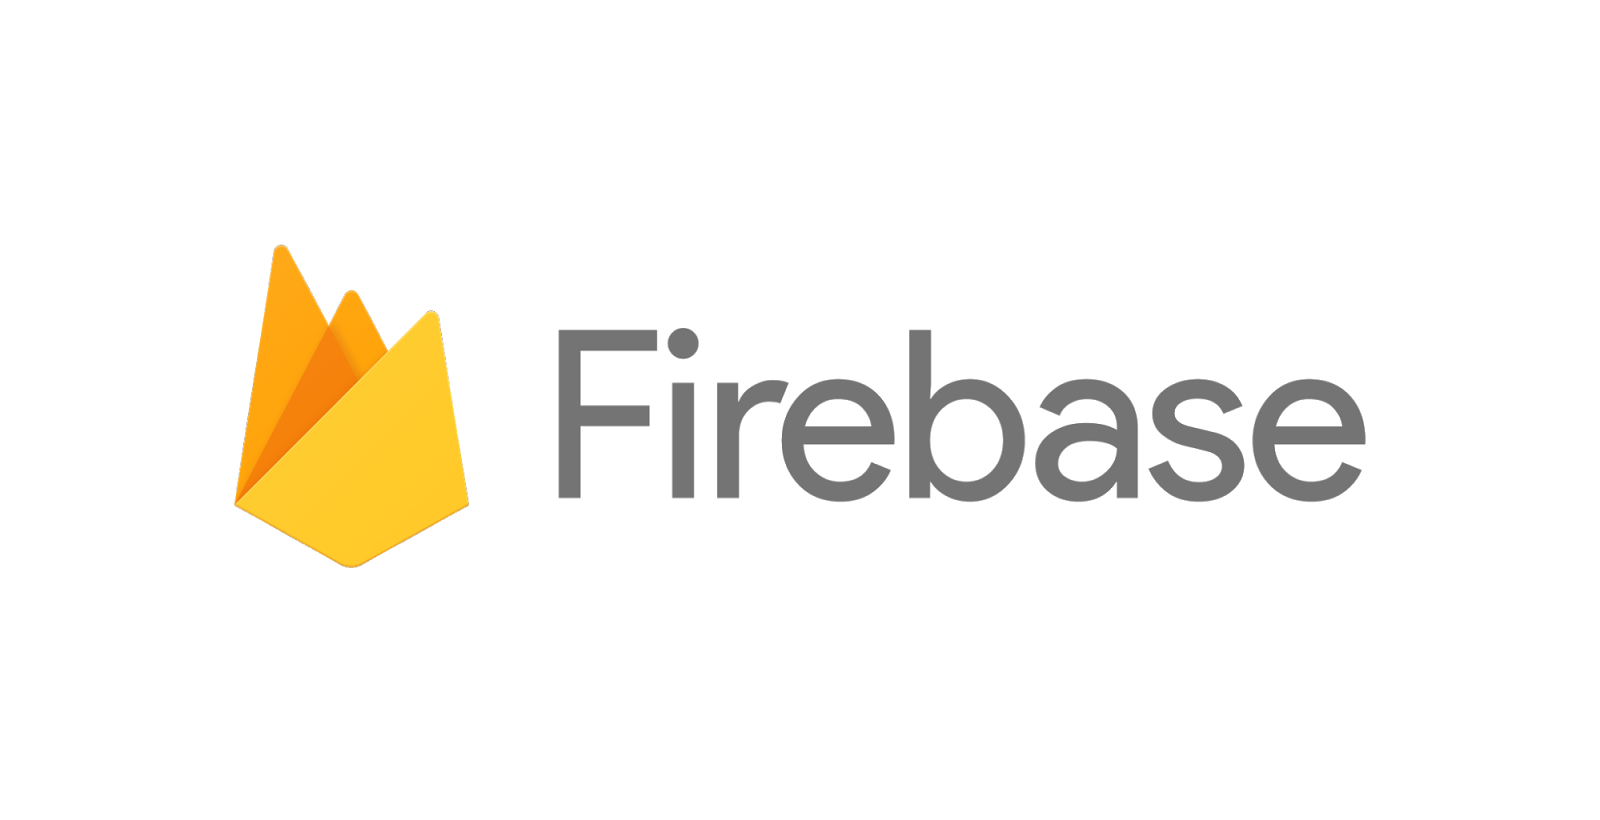
\includegraphics[scale=0.25]{img/firebaselogo.png}
    \caption{Firebase Logo}
    \label{fig:Firebase}
\end{figure}

\subsection{Features Used}
Firebase lets to build more powerful, secure, and scalable apps, using the world-class infrastructure. There are seven different products focused on building a better app. Our project takes advantage of Authentication, Realtime Database, and cloud functions Almost all of Firebase products are extremely useful and are worth mentioning but ill explain only those that we used. we will first summarize the products and then go into further detail on the specific products we used in our project and why we used it etc.
\subsection{Cloud Firestore}
Use NoSQL databases hosted in the cloud to store and synchronize data across users and devices worldwide. Cloud Firestore provides you with real-time synchronization and offline support as well as efficient data query. By integrating with other Firebase products, you can create true serverless applications.we used firestore as our app database.

\subsection{Authentication}
Firebase Auth provides various authentication methods, including emails and passwords from external providers like Google or Facebook, and direct use of existing account systems. Create your own user interface or use our fully customizable open-source user interface.we used firebase authentication to authenticate the app users with their Email and Password.

Firebase is an excellent option for any developer interested in creating a mobile application, finally we will go over the Pros and Cons of choosing Firebase.

\subsection{The Pros of Firebase}
The advantages that lead to why you should choose Firebase as your app backend are as follows \cite{firebaseprosandcons:online}. 
\begin{itemize}
    \item \textbf{Databases} - Depending on the budget, Google offers robust databases to use with your apps. Both real-time and Firestore databases can be scaled in terms of size, suggesting a fully secure managed solution, that still provides you easy access to your data via the firebase console. Data updates and offline access enable the database to be used in real-time applications, and it is also possible to keep multiple databases in sync.
    \item \textbf{Wide selection of products} - Firebase provides a variety of products to make your application work properly. You can choose between real-time databases and data warehouses, store data in the cloud, and build serverless applications with integrated cloud functions.
    \item \textbf{Free to use for small developers} - The price of Firebase was initially free. This way, you can understand whether it is suitable for your application and understand all the nuances. If you have a certain amount of database storage or need a specific product, you can choose a different plan for the required product or storage. You can use the Blaze pricing calculator available on the Firebase pricing page to do this.
    \item \textbf{Good Documentation} - The entire Firebase platform is well documented. Good technical documentation, API documentation, and SDK links make all products easier to use and access. The Firebase product page contains all the information you need about integration, available platforms, manuals, and documentation. , Manual and list of supported technologies.
    \item \textbf{Accessible UI and ease of Integration} - Firebase requires minimal programming language skills and provides integration through the user interface. It is also built into Android Studio to make it easier to use. Although this eliminates the need for complex configurations, anyone can customize the application.
    \item \textbf{Google products} - Firebase's content delivery network (CDN) has been integrated into the Google Cloud Platform and integrated with all Google products. Another benefit of Google’s product is that the company is unlikely to fail or endorse the product often.
\end{itemize}

\subsection{The Cons of Firebase}
The cons of firebase are limited and depend on the scope of your project. Some of the cons are as follows \cite{Downsidefirebase:online}:
\begin{itemize}
    \item \textbf{Limited Support for Ios} - Although firebase is a cross-platform product, it focuses more on the Android mobile platform than Google products. Android Studio seamlessly integrates all Firebase products, such as test labs, authentication, etc., while iOS devices do not provide such integration.
    \item \textbf{Locked into a vendor} - Usually, this is a big problem with BaaS solutions. If the data cannot be ported to another platform, it can be considered fraud.
    \item \textbf{Unpredictable pricing} - Firebase has two price plans one is completely free which is Spark Plan and, which is perfect for newbies to Firebase. Blaze Plan is a pay-as-you-go option for large applications. This is where the problem arises-it is impossible to know in advance how the increase in traffic will ultimately affect prices. The more you spend on the product, the higher the price of Firebase. Plan; growing your business is both a blessing and a curse. Even professional Firebase integrators sometimes struggle to answer customer questions about the future cost of using Firebase.
\end{itemize}

\section{Apptim}
Apptim is a free software for catching critical defects and identifying new performance concerns in apps during development and testing. On Android and iOS devices, the program automatically measures app render times, power consumption, and resource usage, as well as capturing crashes and other data.
\subsection{Features of Apptim}
\begin{itemize}
    \item \textbf{Easy UI} - Apptim's user interface is straightforward and attractive, making it a useful tool. Furthermore, you may discover thorough documentation on its website to guide you through your first steps with the program.
    \item \textbf{Native and hybrid} - Both native and hybrid apps can be tested with apptim but the software only focus on the native part.
    \item \textbf{Performance and bug reports} - After each test session, the tool creates a report that includes performance data as well as a summary for each bug discovered during the Apptim test session.
    \item \textbf{Jira integration} - It connects with Jira via an API key, allowing you to post and track problems directly in this project management application.But this feature is only avaible in paid plans.
    \item \textbf{Test on real devices:} - The tests are performmed on real devices so we have to connect our phone with the pc in which apptim is installed to start testing.
\end{itemize}
\section{why we used Apptim}
we used apptim for performance testing our app as Apptim is free as compared to its competeitors and it adds a lot of value to the Android and iOS app testing process without demanding a lot of effort from the tester or developer.
Every report contains a wealth of information that can be used to detect, mitigate, and prevent risks and issues.
It is a simple tool to implement, straightforward, and simple to use, and it does not necessitate substantial performance understanding.
\chapter{System Design}

\section{Chapter Introduction}
In this section, we will discuss the architecture of the application. The
components of a flutter application and how the Front-End communicates with the Back-End.

\section{System Architecture}
\begin{figure}[!htb]
    \centering
    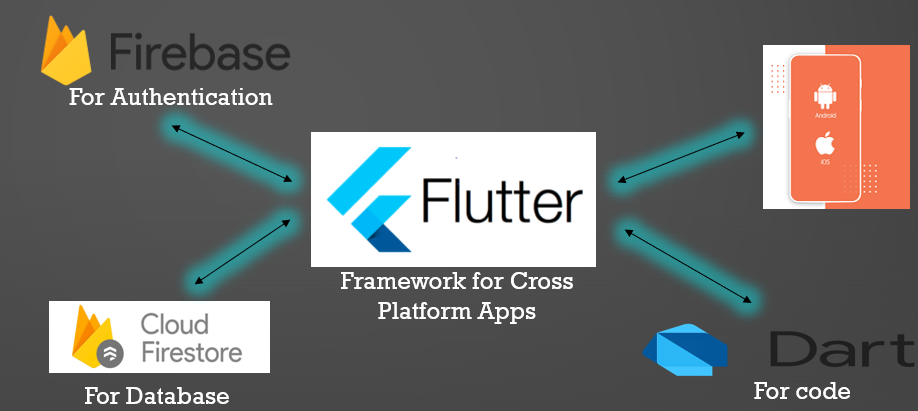
\includegraphics[scale=0.70]{img/systemArchitecture.PNG}
    \caption{System Architecture}
    \label{fig:System Architecture}
\end{figure}

\section{Project Setup}
First we Installed flutter from "flutter.dev", Android toolchain, and Android studio. we didn't install Vs Code as we already had it in our systems. After installing the above we checked-in command-line window by typing "flutter doctor" that all are the boxes are checked and no issues found in the doctor summary and finally installed an extension of flutter in Visual Studio Code. 

First created a new firebase project and then Created a new flutter project and added all the required assets for the project in "pubspec.yaml". 

Then we created a project in firebase and added an android app filled in app registration details such as android package name, app nickname and sha keys and then added the firebase sdk into the build.gradle file of our flutter project and then downloaded and added google-services.json file to our project 

Next we enabled Email and Google login from Authentication sign-in method tab.
\section{Splash Screen}
When a user first opens the app an animated splash screen with the app name is displayed to the user.
\begin{figure}[H]
    \centering
    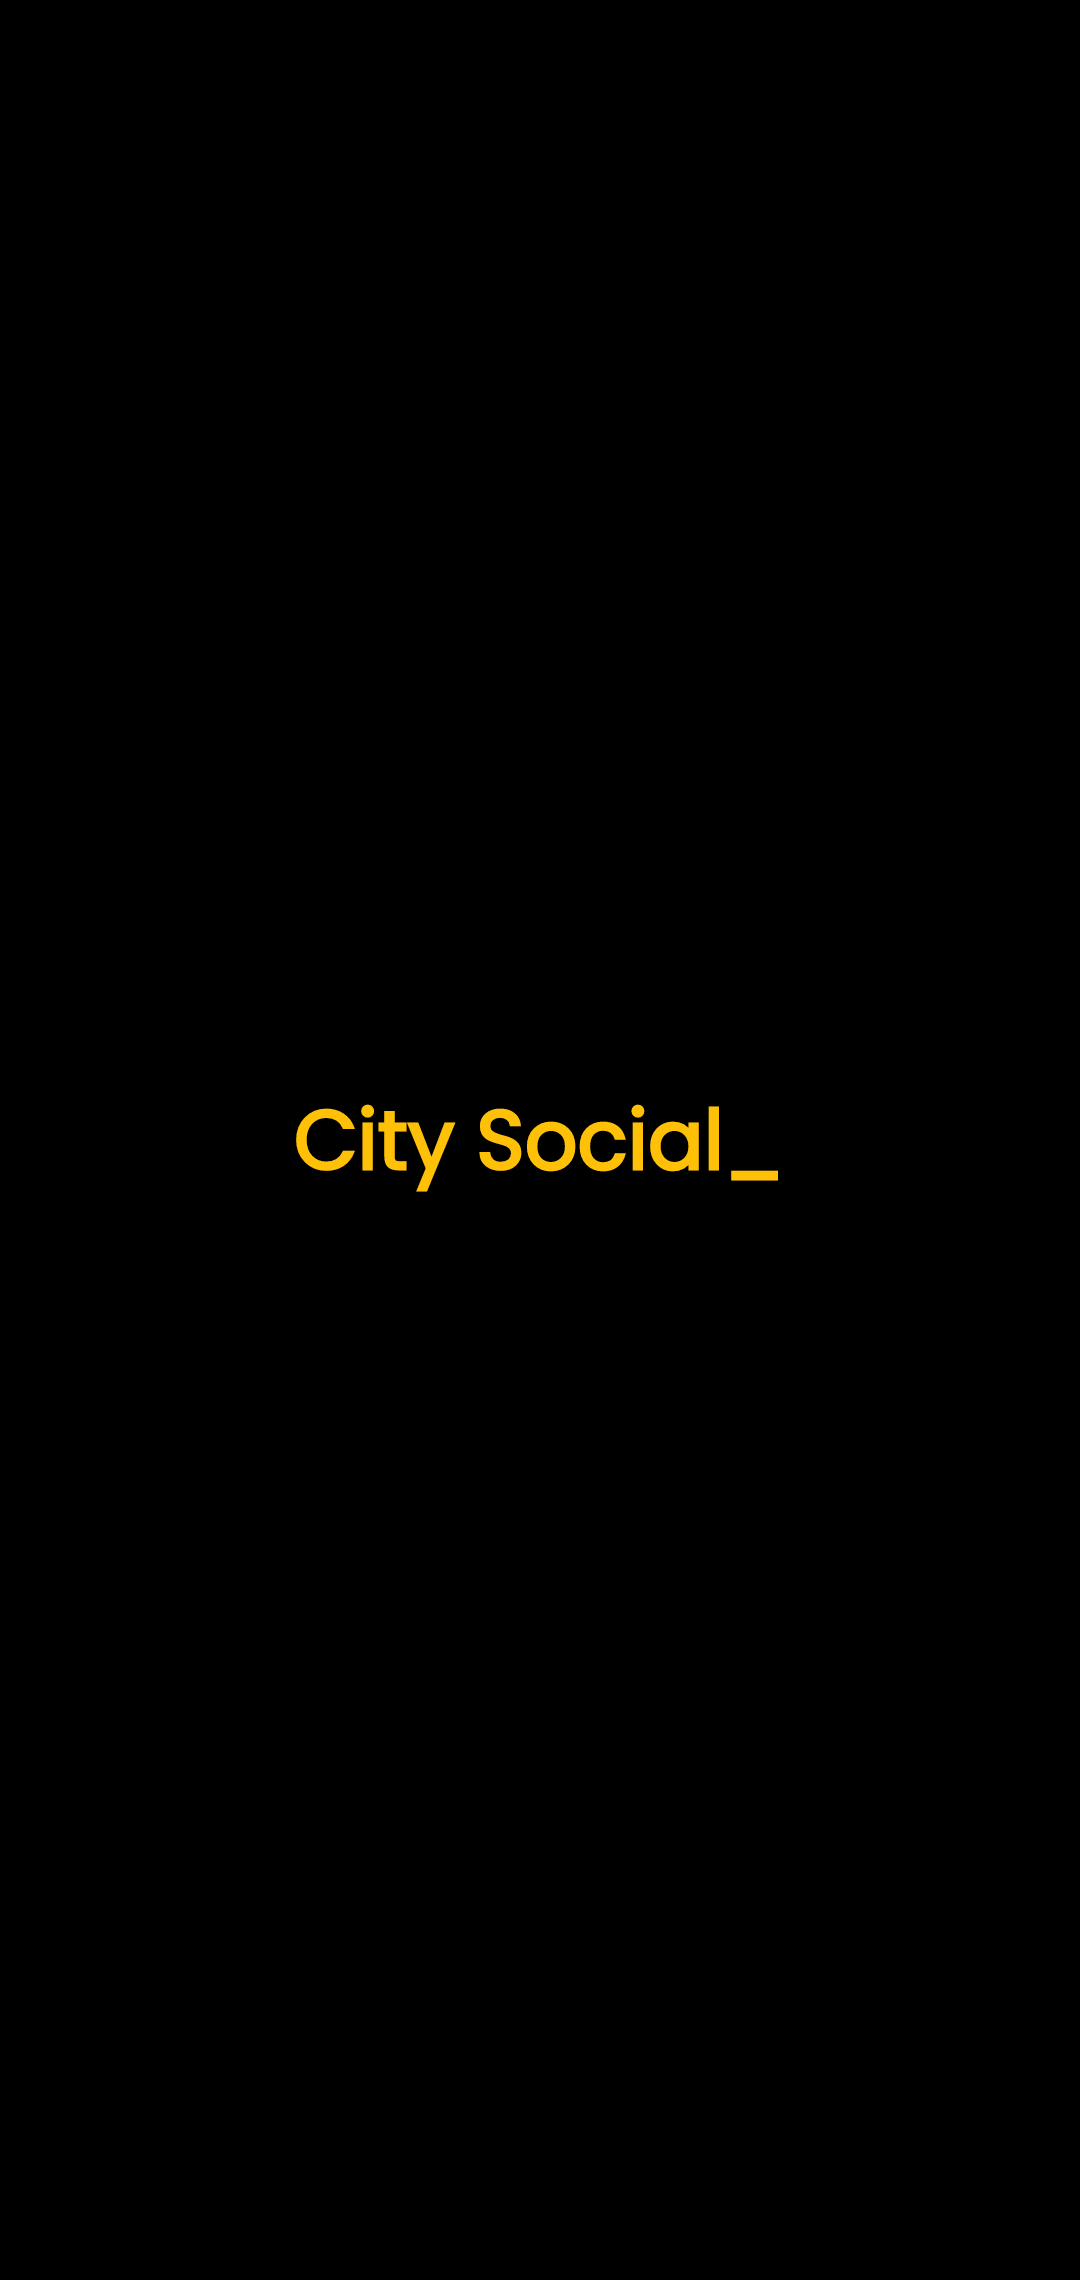
\includegraphics[scale=0.10]{App Screenshots/SplashScreen.png}
    \caption{Splash Screen}
    \label{fig:Splash Screen}
\end{figure}
For this we created a new class called splashscreen.dart and imported "animated-text-kit" library of flutter to use prebuilt animations for building animated splashscreen.

We created a widget positioned in the centre and used the \textbf{TypewriterAnimatedText} widget and set its colour to yellow and duration of 150 milliseconds and in initstate function we tranisitioned the page after 3 seconds to the welcome screen.

\section{Welcome screen}
After SplashScreen timeout user is taken to the Welcome screen where we have the welcome message and a social image attached to a widget.Then we have an Email Button that when clicked presents user with sign in options.

\begin{figure}[H]
    \centering
    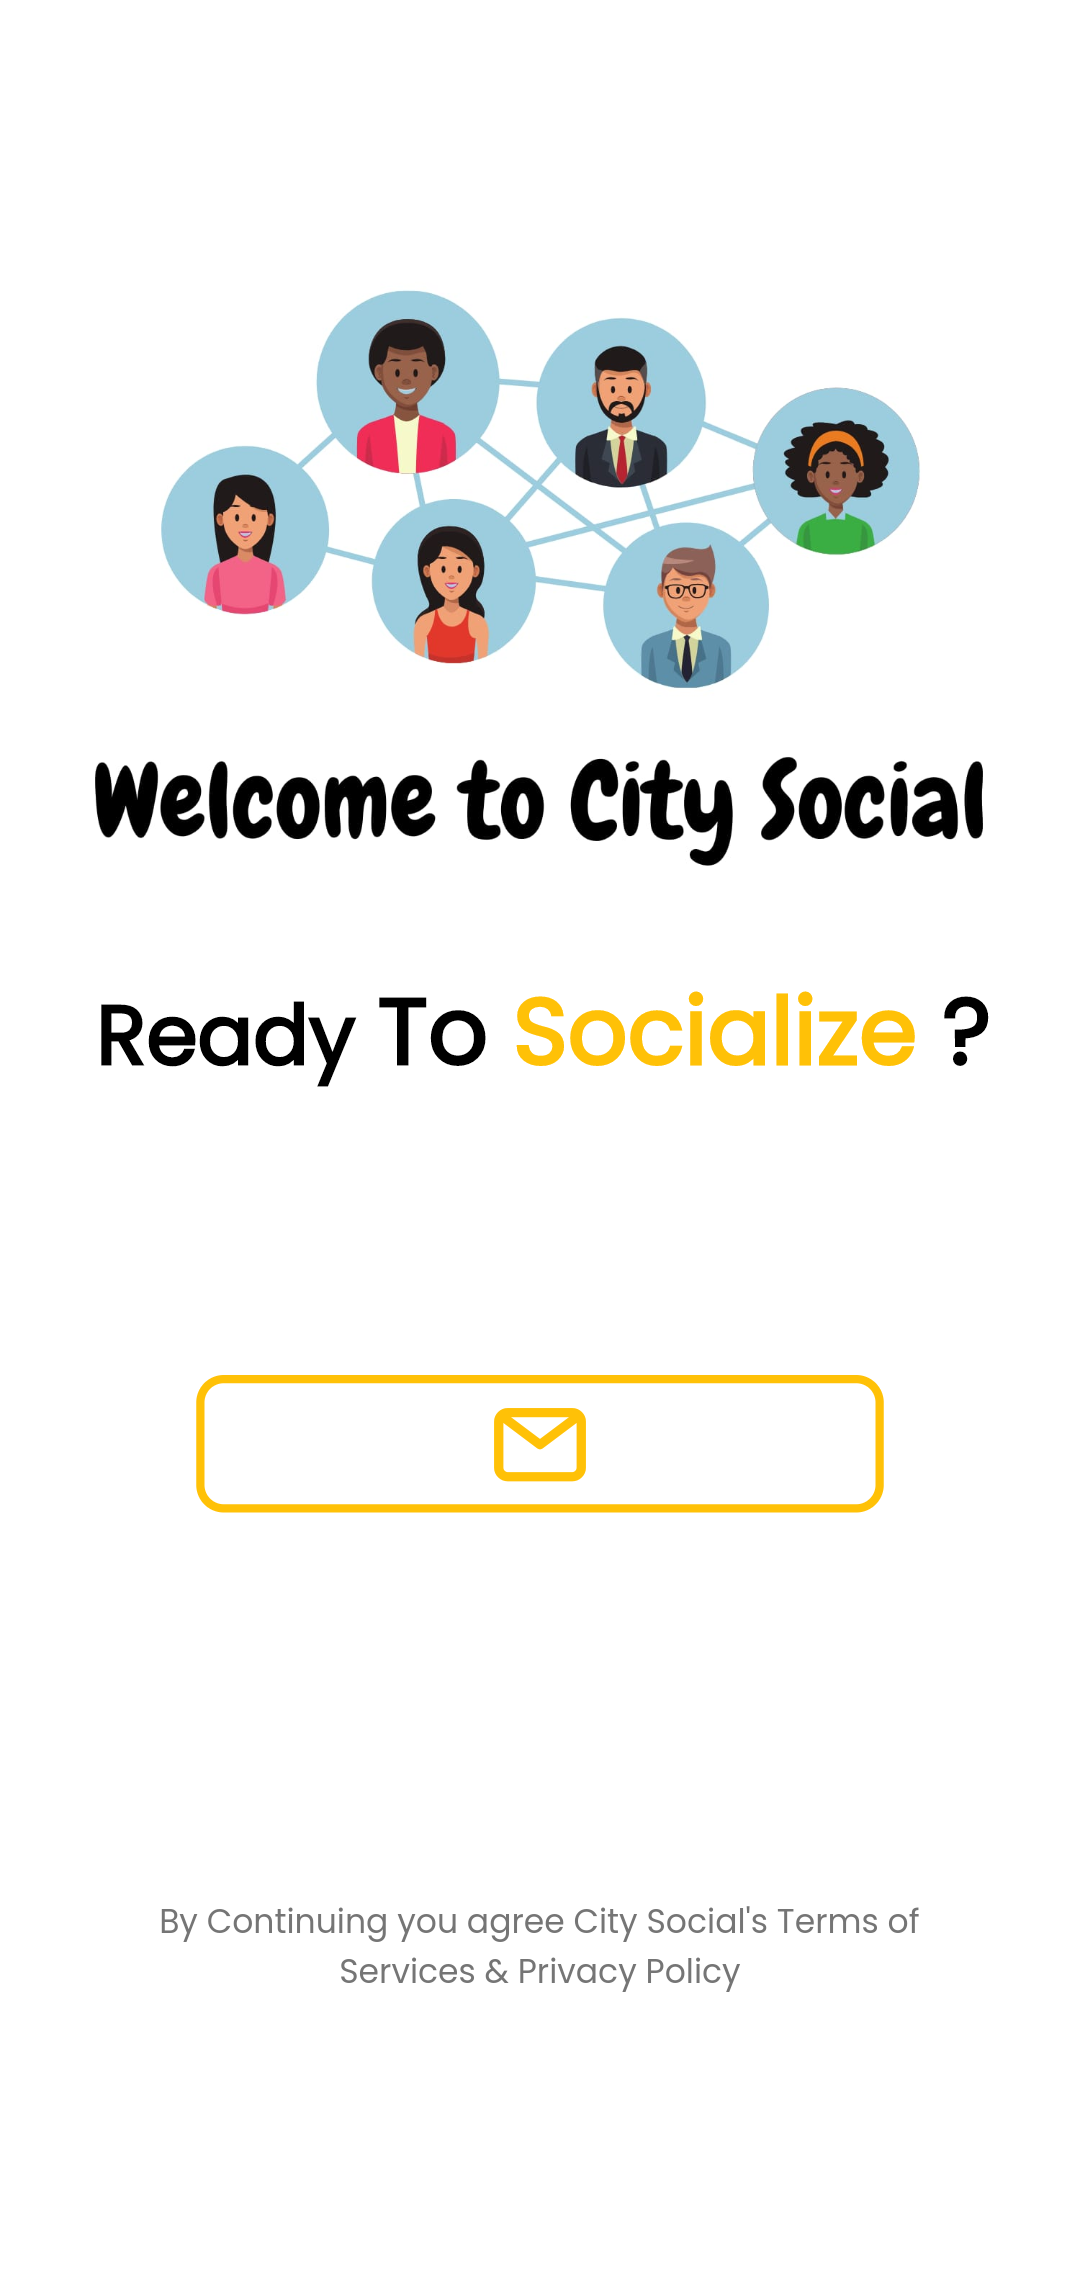
\includegraphics[scale=0.15]{App Screenshots/WelcomePage.png}
    \caption{SignIn Splash Screen}
    \label{fig:Welcome Screen}
\end{figure}

For this we created a stateless class called WelcomePage and to use the state management in our application we used provider state managements.There are other ways of managing the application state as well but after research we found that provide is used used for basic application where more screens have to be managed.

So we imported provider dependency in pubspec.yaml file and created a new class called WelcomePageHelpers to help the state management of WelcomePage. In the helper class we created a bodyImage widget for the background of the welcome screen and imported the image from assets to be used within it.Then we used the provider in the main widget "scafold" of the WelcomePage to get the image.

Then in the helper class we created a widget for the welcome message and tagline and terms\&condition text at the bottom. we used provider in the WelcomePage to get it displayed on the welcome screen.

Then same as above we created buttons in the helper class for Signing in with Email and used the provider in WelcomePage to get it

\subsection{Sign In \& SignUp}
we created a widget that returns a sheet with 2 buttons for sign in for signing in with existing account email and password and signup button for new users to signup.
\begin{figure}[H]
    \centering
    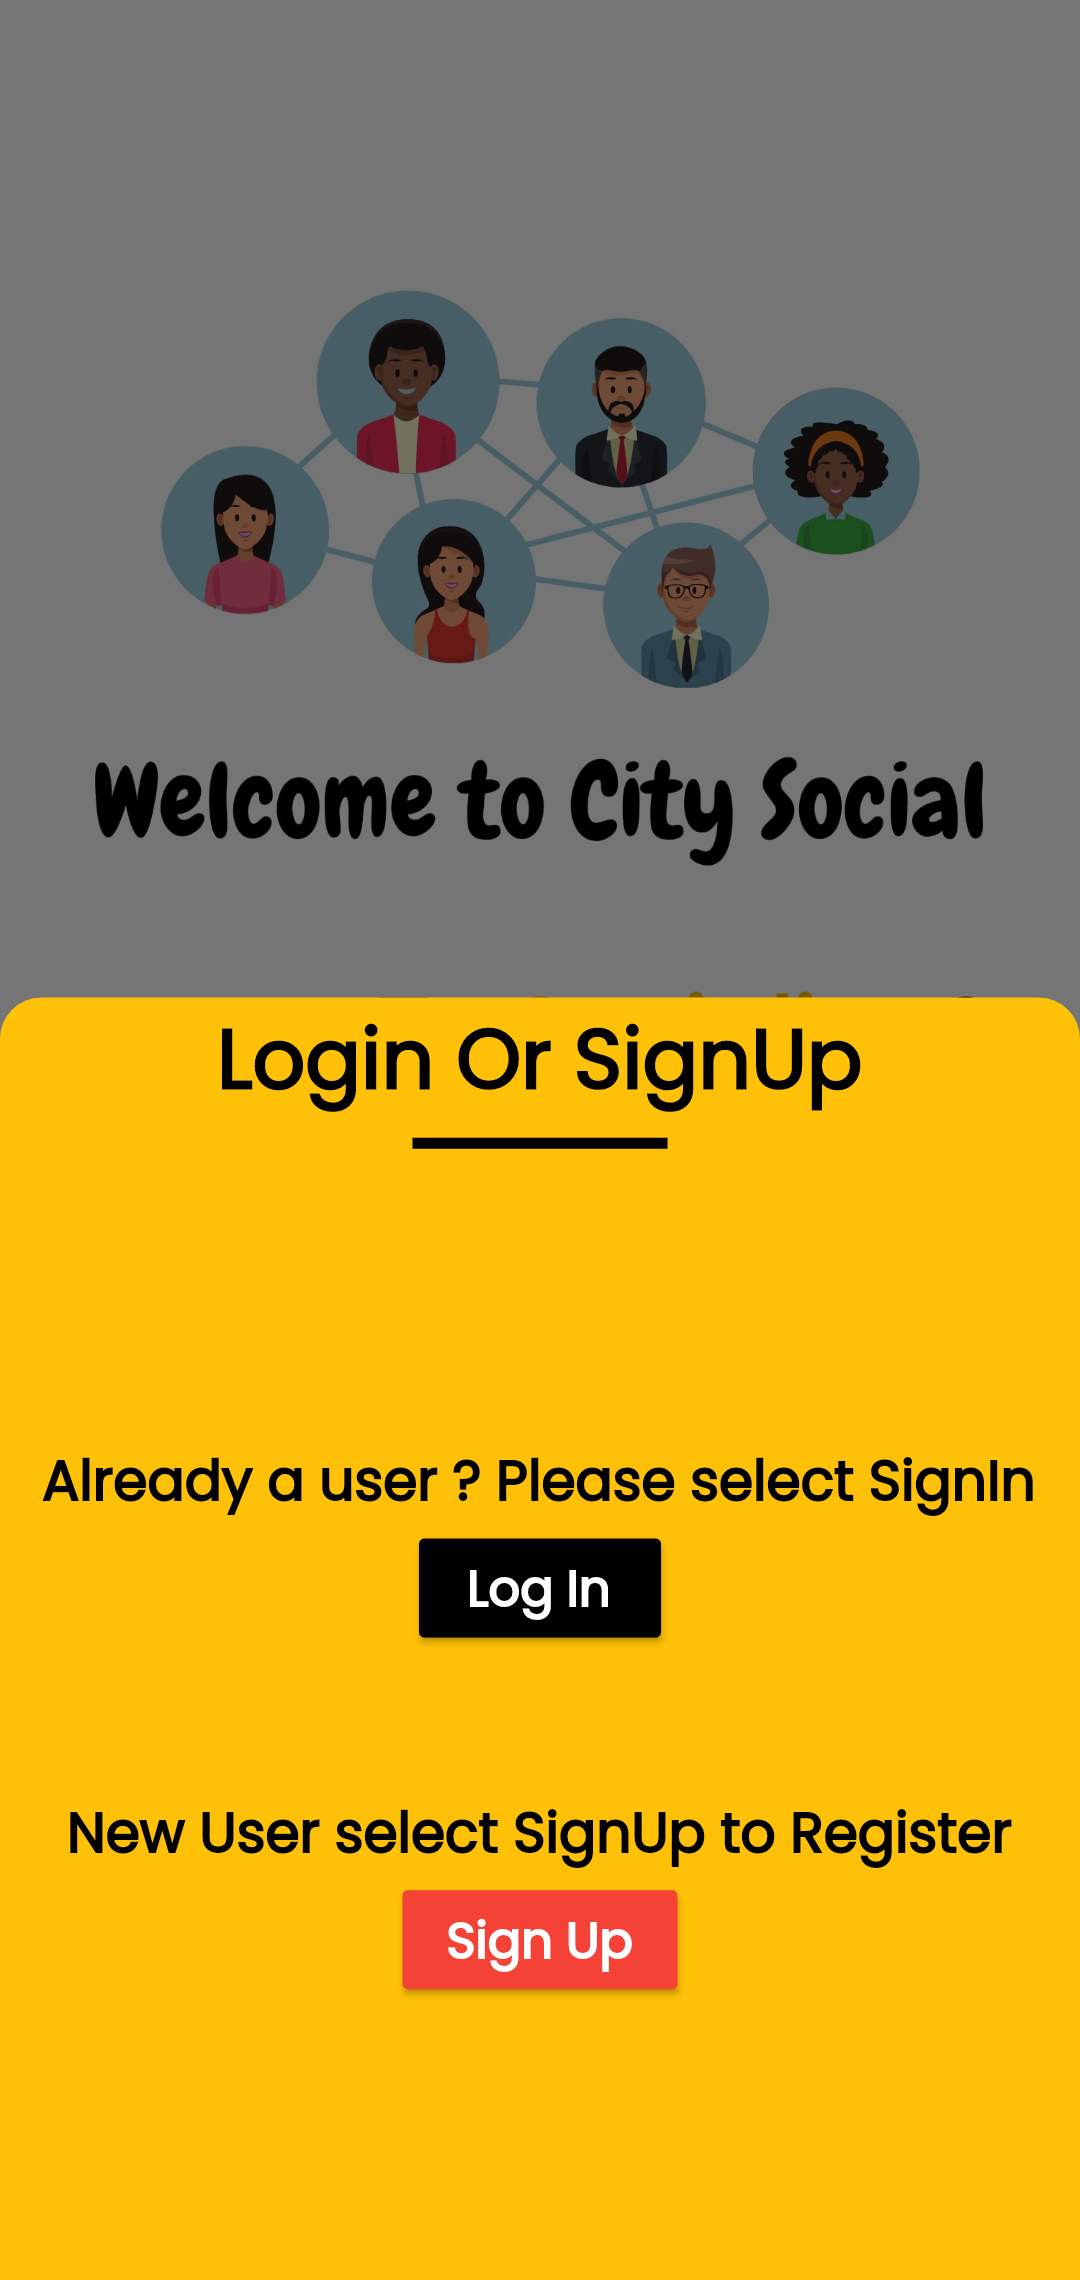
\includegraphics[scale=0.10]{App Screenshots/Login or Signup Page.png}
    \caption{Login or Signup Screen}
    \label{fig:Login or Signup Screen}
\end{figure}
Then we created a Class with changeNotifier feature of provider called WelcomePageServices that contains functions for both signin and signup functionality.

we created a widget for signin form in which we created 2 form fields for entering user email and password for that we created 3 TextEditingControllers and created a action button for signin and ontap we called a function logIntoAccount using provider that we created in a class called authentication.It is an asynchronous function that uses the signInWithEmailAndPassword of firebase to check user details and login.
\begin{figure}[H]
    \centering
    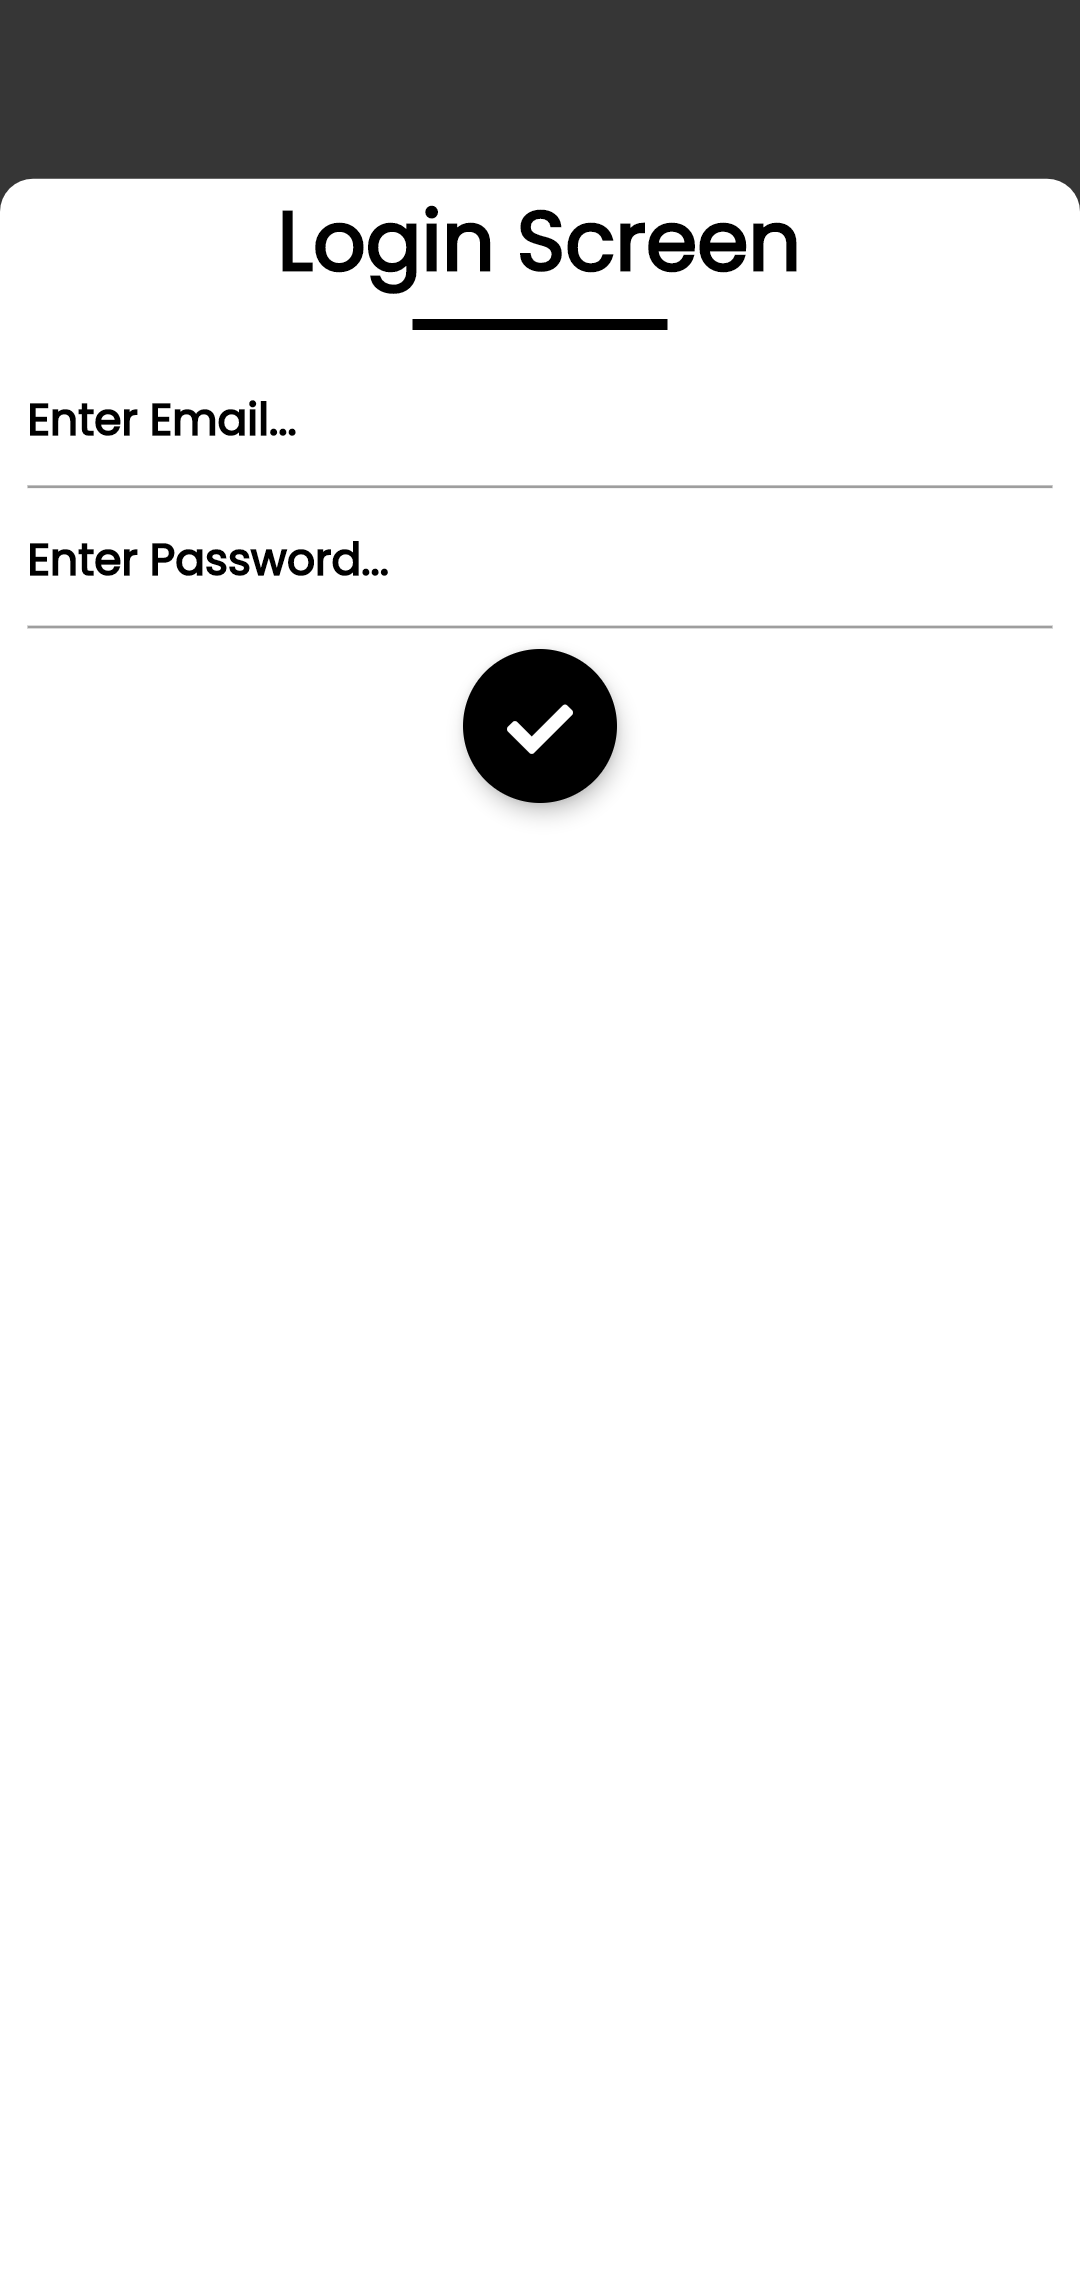
\includegraphics[scale=0.15]{App Screenshots/Sign-In Screen.png}
    \caption{SignIn Screen}
    \label{fig:Sign-in Screen}
\end{figure}
Similarly we created a widget of signup form and action button which when tapped after entering the required information calls the CreateAccount async function from authentication class using provider to use the createUserWithEmailAndPassword function of firebase to signup and calls CreateUserCollection method of firebaseOperations class to create a collection in cloud firestor which stores userid,username,useremail,userPassword and userimage.
\begin{figure}[H]
    \centering
    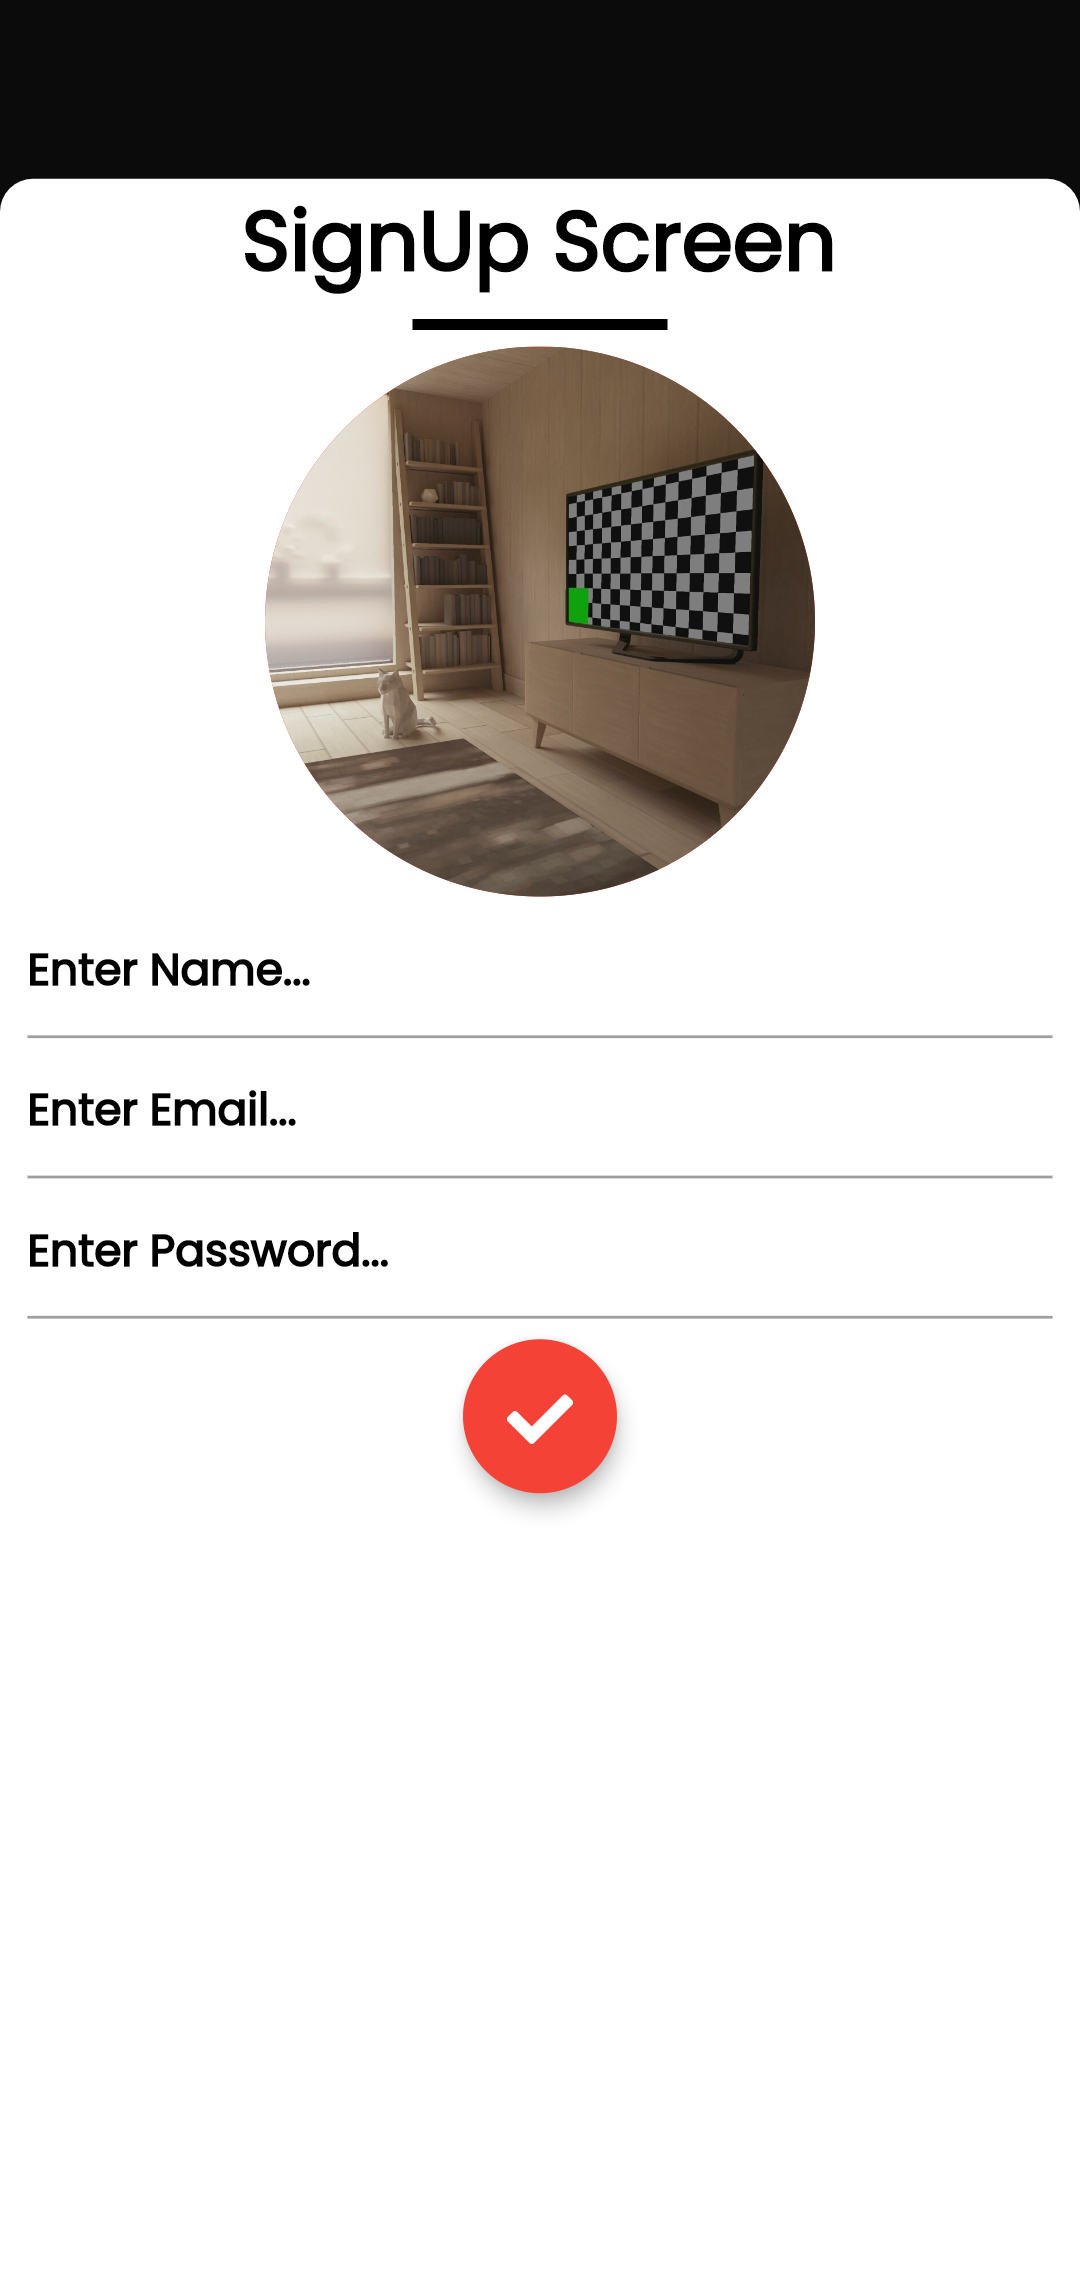
\includegraphics[scale=0.11]{App Screenshots/Sign up Screen.png}
    \caption{SignUp Screen}
    \label{fig:Sign-up Screen}
\end{figure}
After successful login or signup the app navigates to the homescreen.

\subsection{Display Image}
When user clicks on the signup button two buttons a shown to the user one is called camera to capture the image from camera and the other is gallery to select an image from gallery as a display picture for profile.

so for this we created a new class under a Backend folder called firebaseoperations and created an asynchronous function called "pickUserAvatar" which gets the path for the picked image by the picker and then we created a widget in the WelcomePageServices page to show the user display image by using CircleAvatar and using the provider to get the image url from the getUserAvatar method of landing utills through provider to be shown as the background image.

Then after selecting an image user is presented with two options of buttons to reselect or confirm the image so for reselecting we define in the ontap function to call the pickUserAvatar function of WelcomePageUtils through the provider to reselect the source image. For confirming the image we created a asynchronous function in firebaseoperations class to upload the selected image to the firebase so we used reference class of firebase storage for reference to the firebasestorage where the image will be stored along with its path and time stamp and used the uploadTask class of firebase storage to upload the image to firebase storage then we get the url of uploaded image through getDownloadurl method of firebase storage and assign it to the userAvatarUrl.

\section{Timeline Page}
The is the first screen where user is taken to after successful login.It has and appbar with camera icon on the right side which when tapped shows two buttons one for gallery and one for camera.The gallery button when tapped takes to the gallery of the phone to select an image from there and the camera button open the phone camera app to take the picture.After that reselect button and confirm button shows up and if user selects reselect it takes user to the previous screen to select image again and if user taps confirm then a caption screen is displayed where user can write caption and after pressing the share button the image is stored in the cloud firestore and is displayed in timeline feed.
\begin{figure}[H]
    \centering
    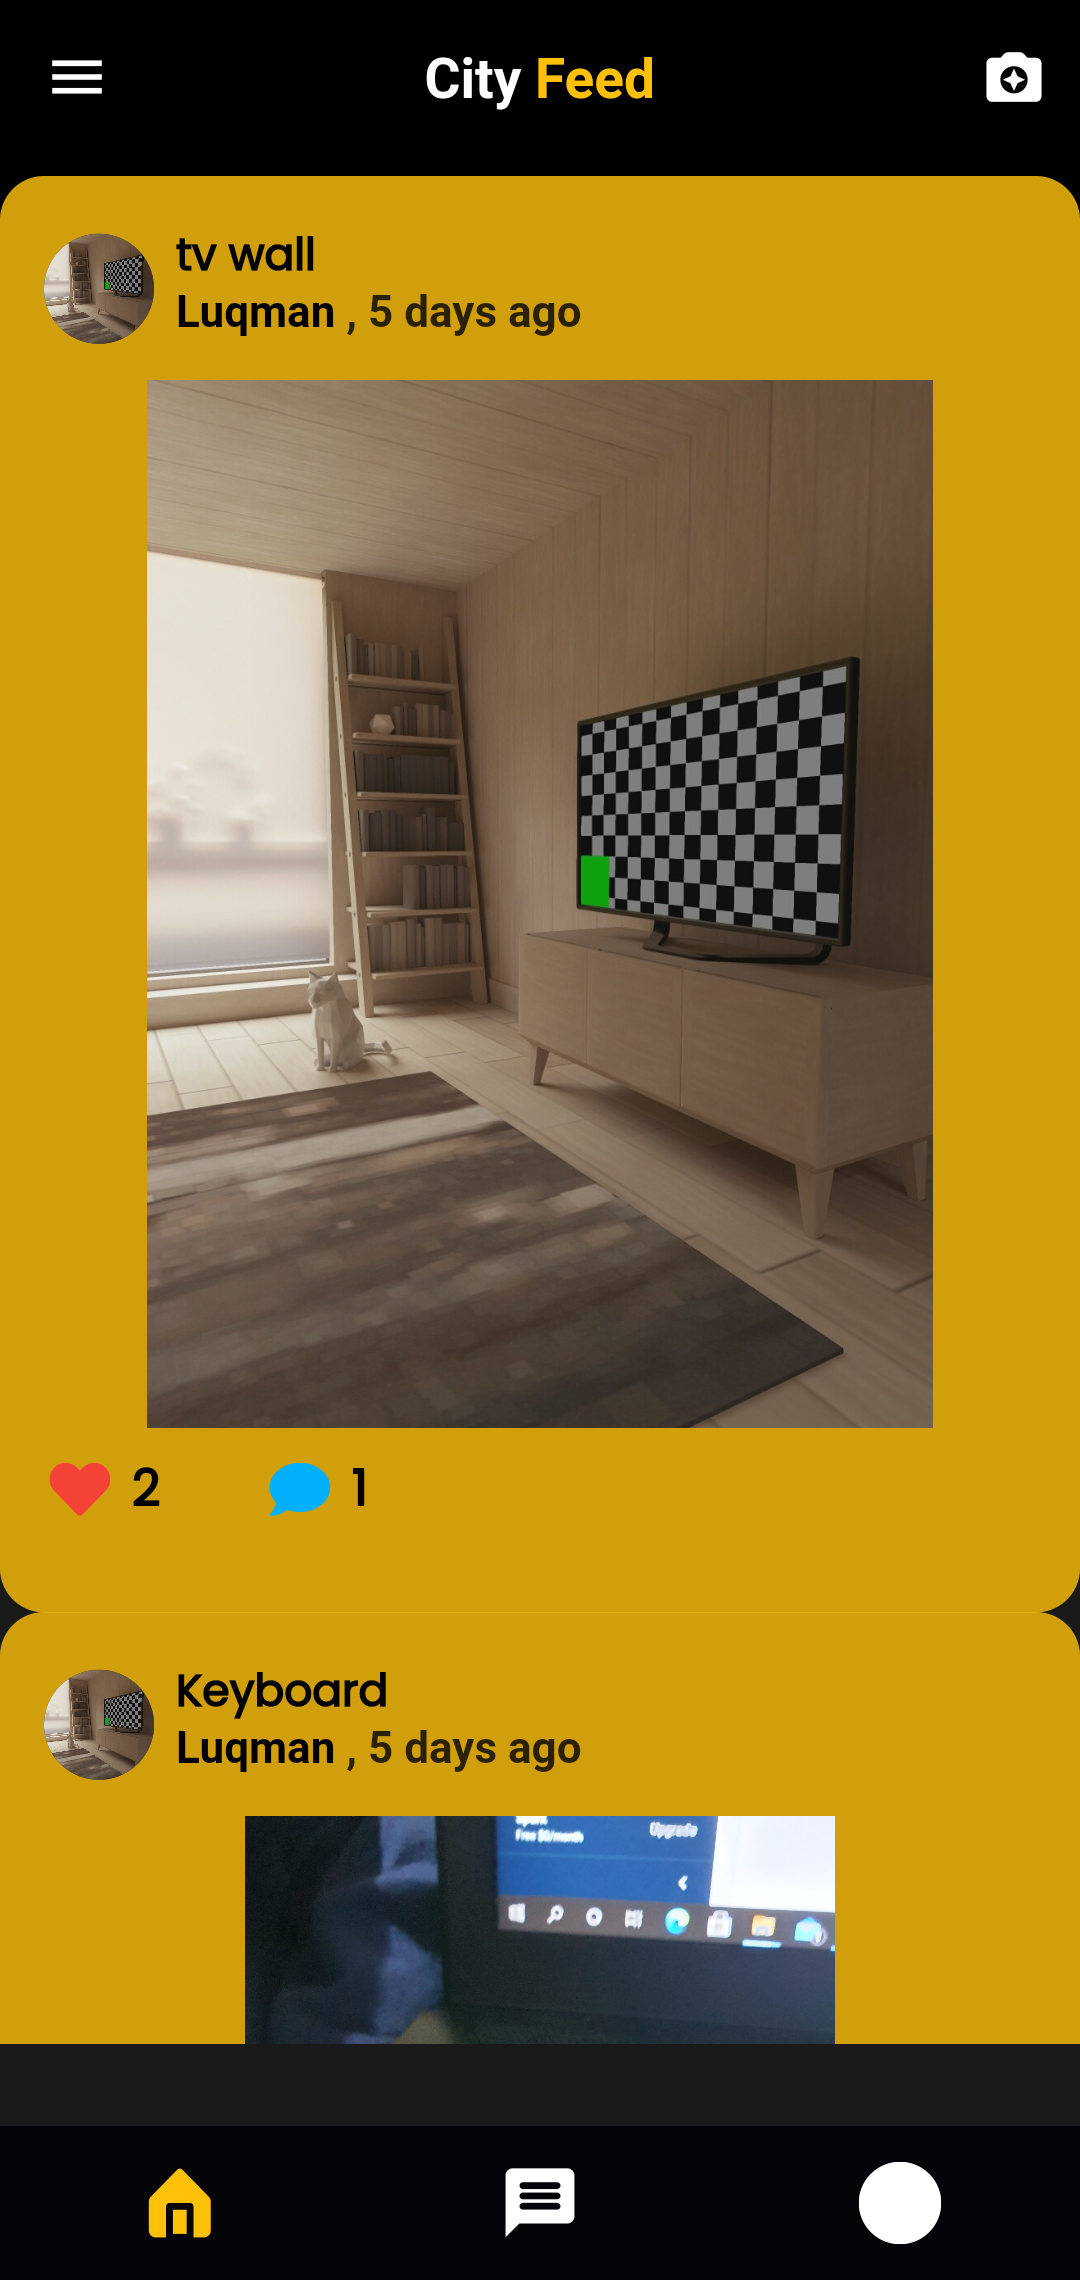
\includegraphics[scale=0.10]{App Screenshots/Timeline Page.png}
    \caption{Timeline Screen}
    \label{fig:Timeline Screen}
\end{figure}
\subsection{Upload Post}

For Uploading post we created a class called UploadPost and created a widget called selectPostImageType for gallery and camera options and used the provide to call them in FeedHelpers class of timeline page.

For selecting image we created a asynchronous method called PickUploadPostImage in which we have an "uploadPostImageval" variable which is waiting for the picker to get the image from the source which is depending upon the imagesource that we provide and then assigning the path of that image to UploadPostImage file.

For Uploading the image we created a Future async method called UploadPostImageToFirebase in which we a reference to our firebase storage with our image path and used UploadTask method of firebase to store it in firestore collection called "posts".

We Created another widget for caption of the post and called the image editpostsheet and used UploadPostImageToFirebase method to upload the image to firestore and created another method in firebaseOperations class called UploadPostsData to handle the upload data along with its caption and called that method in the ontap function of share button in the ontap function of editpostsheet widget share button.

\subsection{Timeline Posts}
On Social Feed page / Timeline page all posts from all users are displayed which are vertically scrollable so to implement that we will use stream as it is a continous flow of data.so we used a streambuilder widget and defined the source to firestore collection of posts.

Then we created another widget called loadposts to structure the posts to display them in the feed with profile image of post owner its name, caption, timestamp and buttons at the bottom of each post for like and comment functionality.

Then we called this widget in the feed body to display the posts.

\subsection{Delete Post}
There is a 3 doted button beside every post which when tapped shows the option to delete a post .
For this functionality we added a method in the PostFunctions file in which we created a button for delete post which when tapped ask user with 2 options "yes" or "no" to delete post and tapping on yes invokes the delete method that we created in FirebaseOperations class to delete user data by using the delete fuction of firestore.

\subsection{Like Posts}
For Likes Functionality we created a new class for it called PostFunctions in a file called PostFunctions. In that class we created a new asynchronous future mehtod called addLike what creats a subcollection called likes in the posts collection and then storing data of the user who liked that post in that collection.

There is a heart shaped button under each post which when tapped calls the addLike method of PostFunctions class using provider.And to display them we called the snapshot of document data in the text field of the heart widget.

\subsection{Likes Information}
On Long pressing the likes button a sheet is displayed that shows all the users info who liked that post and in front of them a Follow button to follow them.

\begin{figure}[H]
    \centering
    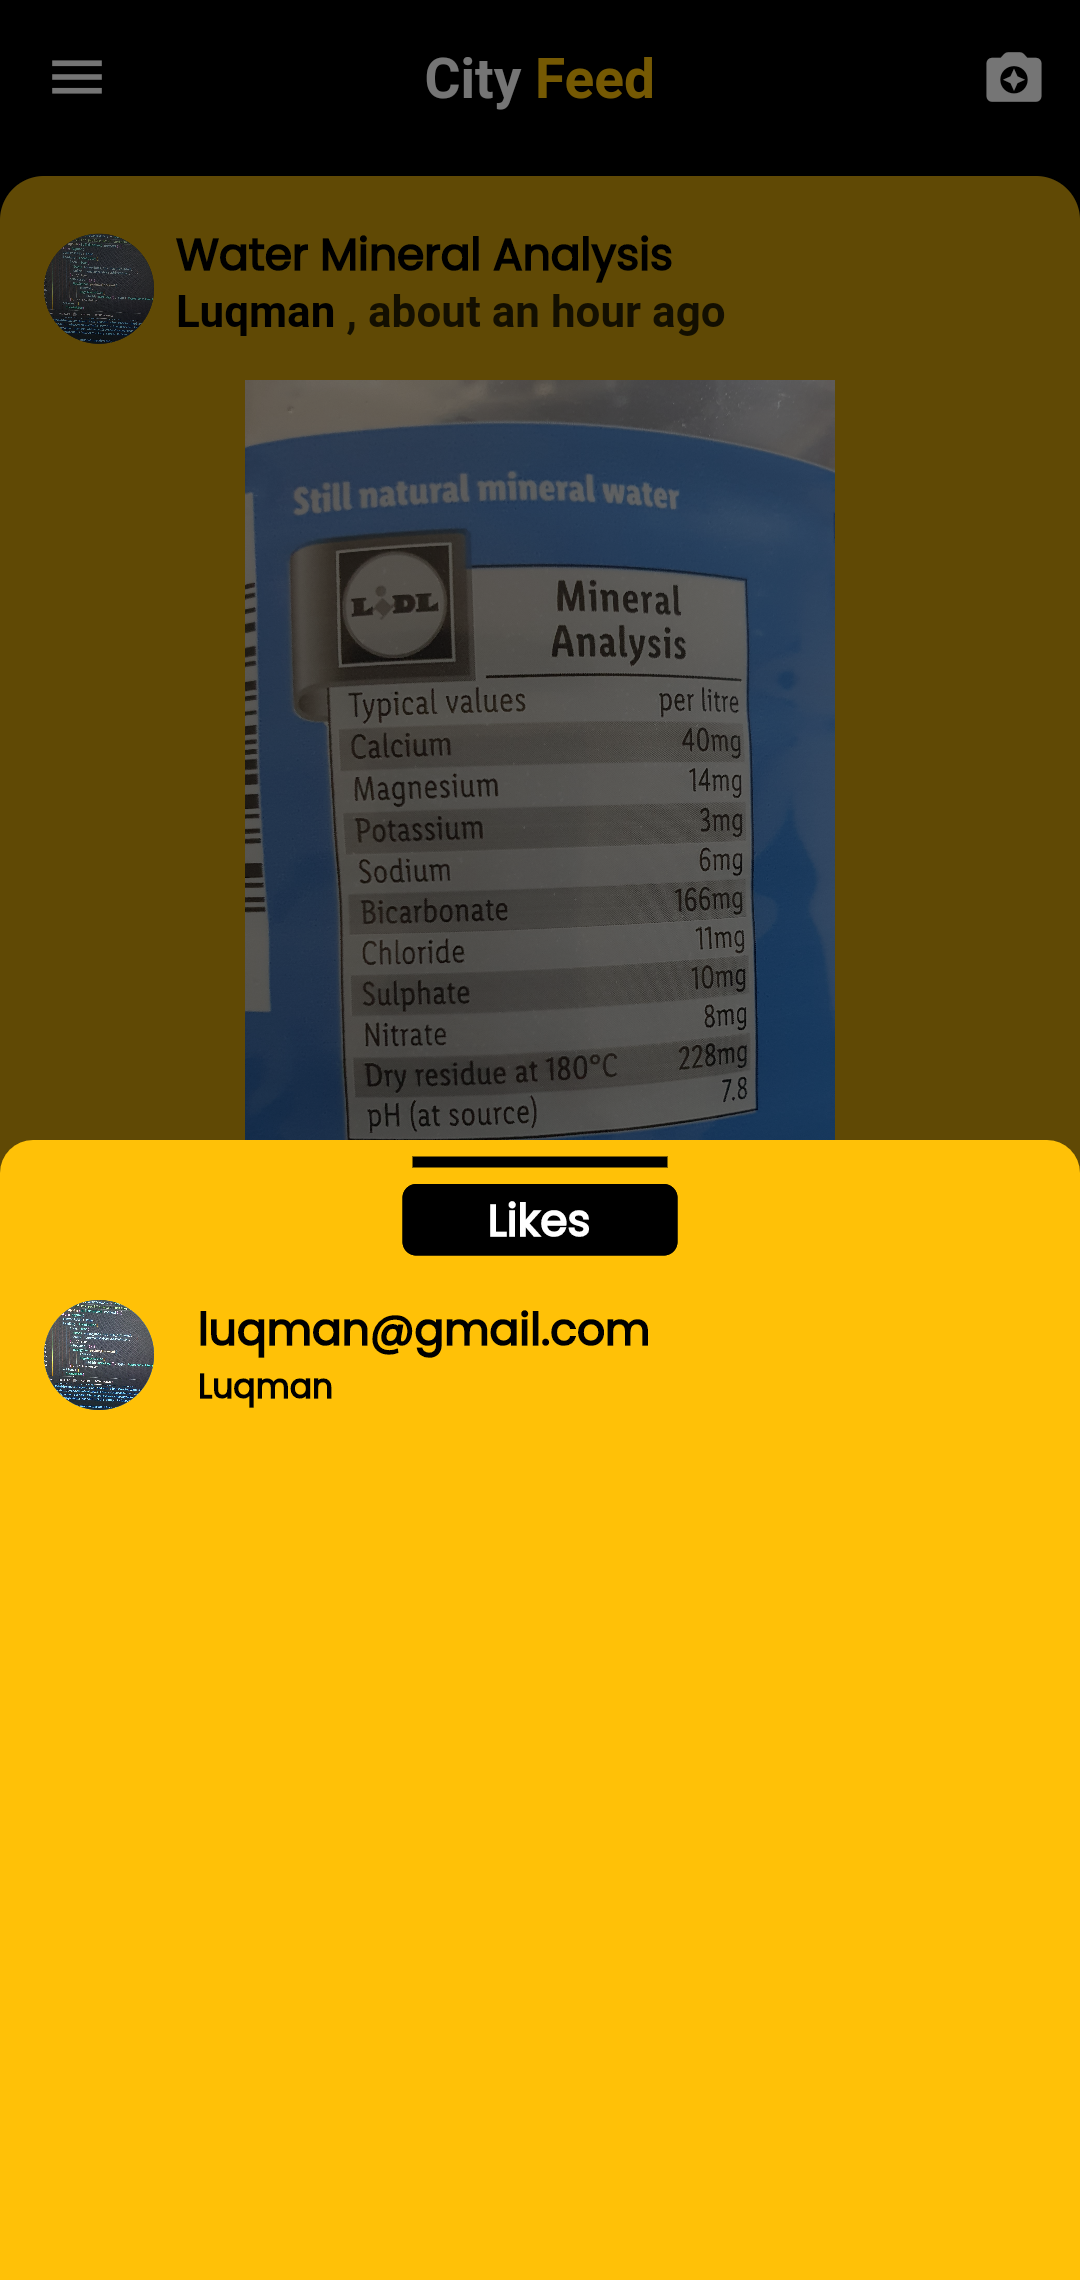
\includegraphics[scale=0.12]{App Screenshots/LikesInfo.png}
    \caption{Likes Information Screen}
    \label{fig:Likes Information Screen}
\end{figure}

To implement that we created a method called showlikes in PostFunctions class and used the stream to fetch data such as username,useremail,likes,Time from likes collection of firestore and used builder to show them in listview.

\subsection{Realtime Messaging with Comments}

For Comments we Created an asynchornous method called addComment that creates a subcollection of comments under the postId document of posts collection and under that it creates a document which contains the comments data such as comment,username,useruid,userimage,useremail,timestamp etc

To Add the comments we created another method called showCommentsSheet that returns a widget with a sheet on which comments are displayed and there is a text field for writing text with a hint text add comment... and ther is an action button beside text field which when tapped calls the add comment method to store comment in firebase.

To display comments we used the stream from comments collection of firebase firestore and order it by timestamp and return it in the listview using builder and called it in loadposts method using provider.

\begin{figure}[H]
    \centering
    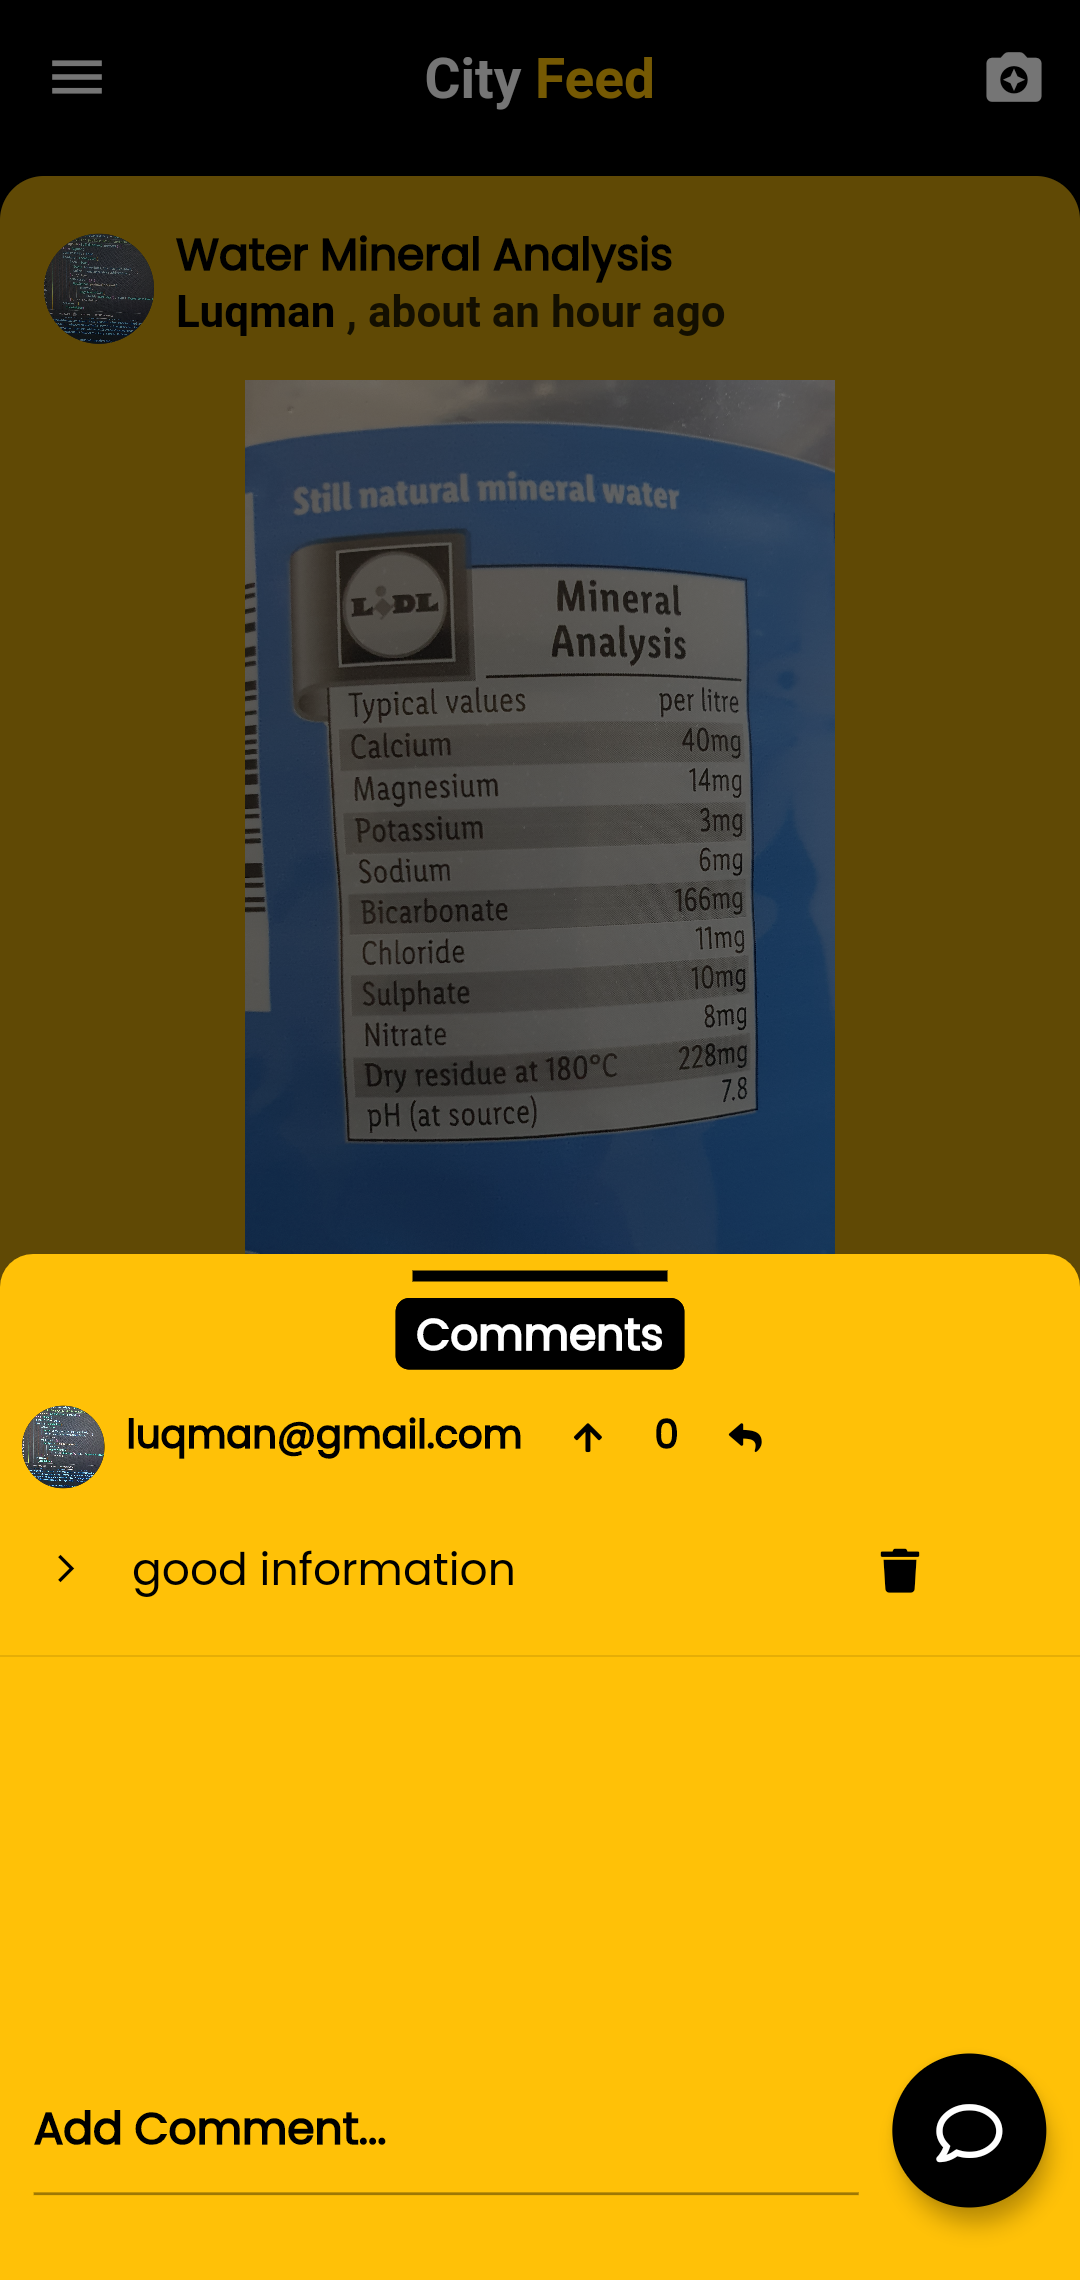
\includegraphics[scale=0.14]{App Screenshots/Comments.png}
    \caption{Comments Screen}
    \label{fig:Comments Screen}
\end{figure}

\section{Profile Page}
When user clicks on the profile picture at the bottom navigation bar it is taken to the profile page where we have user profile picture displayed at left side along with the number of posts , followers and following.There is a section of recently added in which the recent posts of users whom a user follow are displayed.We also have the user posts displayed below them.
\begin{figure}[H]
    \centering
    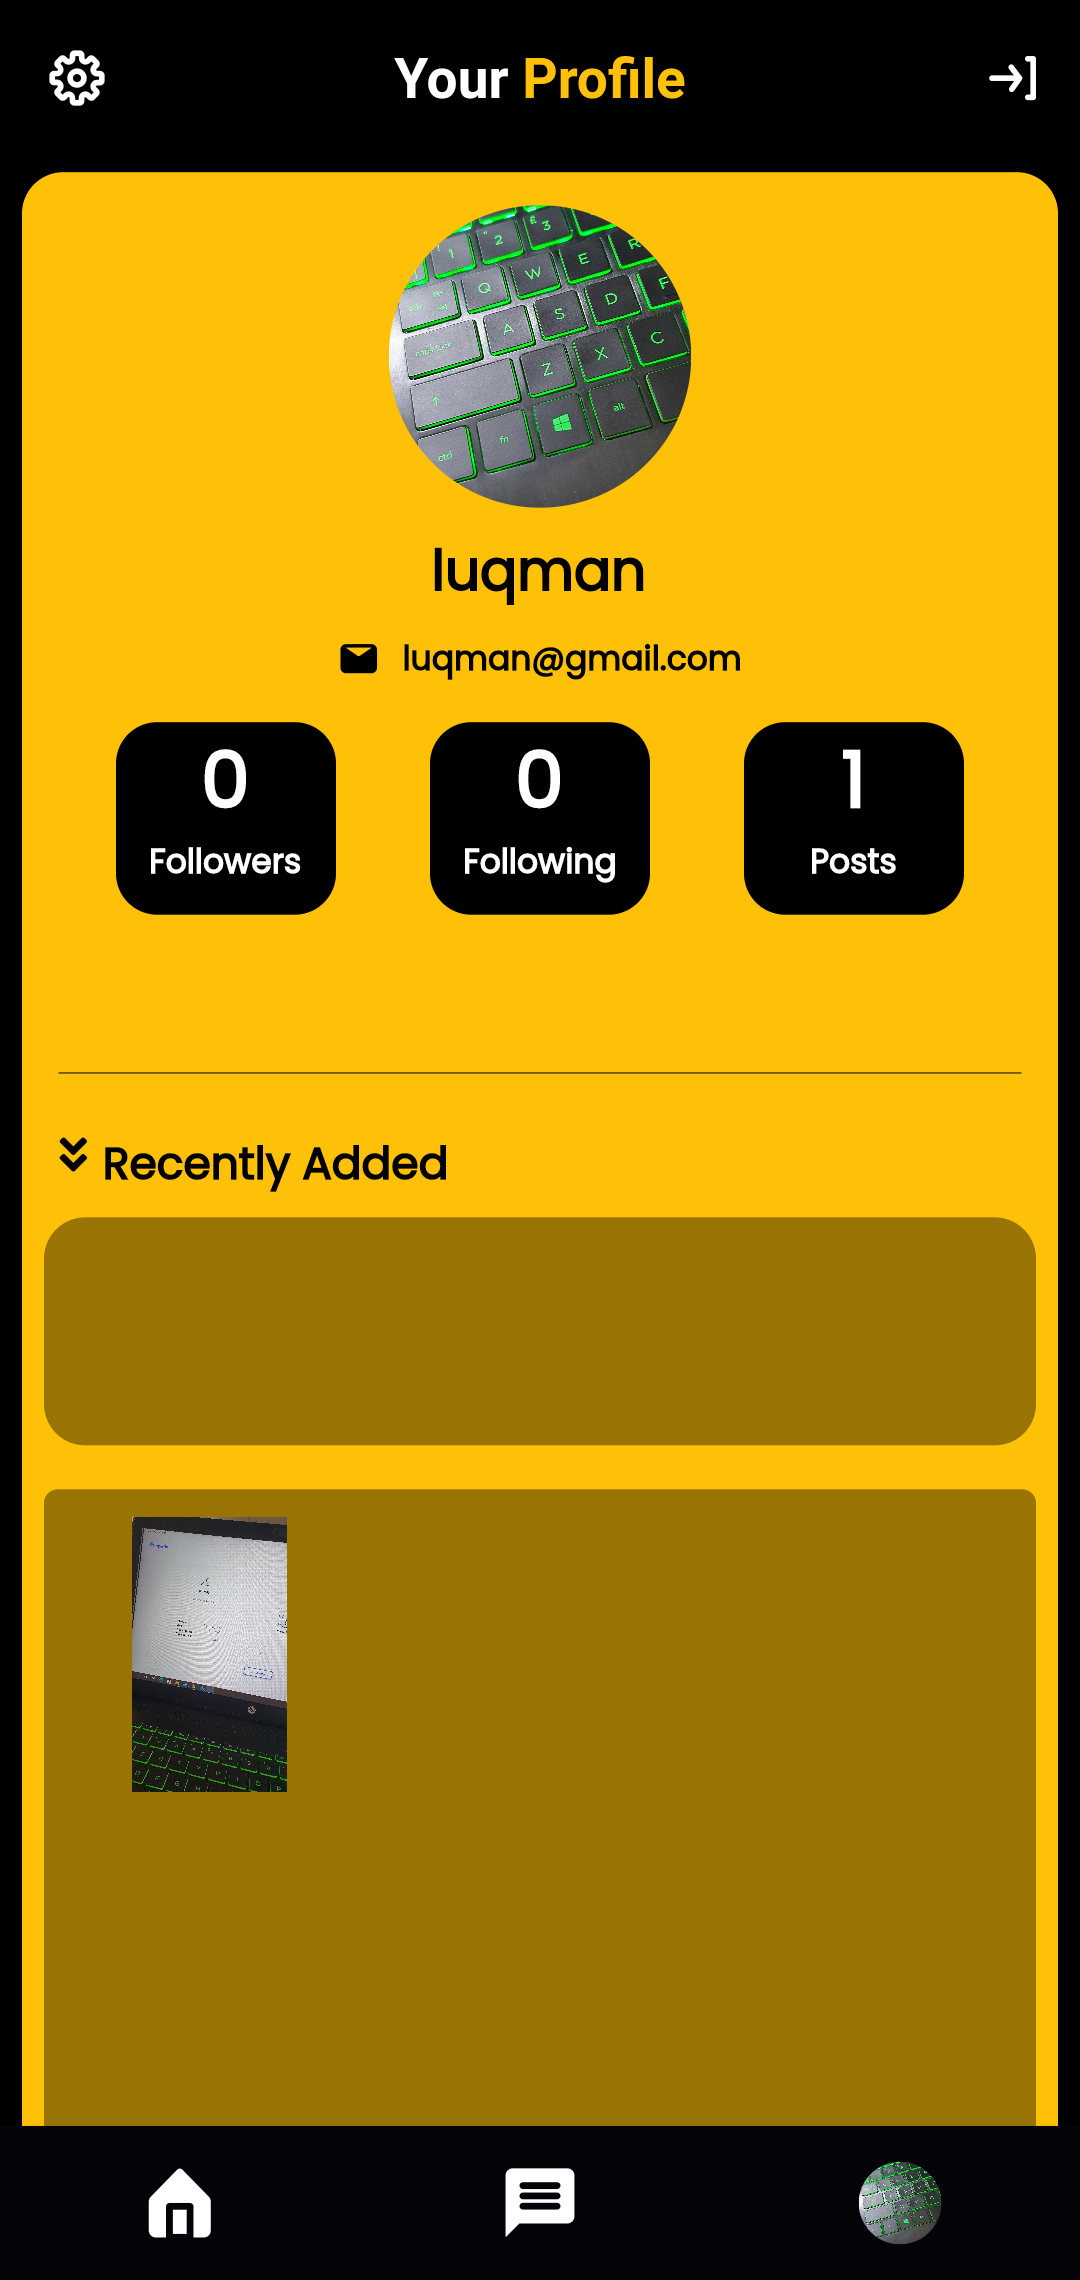
\includegraphics[scale=0.13]{App Screenshots/profile Page.png}
    \caption{Profile Page}
    \label{fig:Profile Page}
\end{figure}
For this we created widgets in new class called profileHelpers in which we fetched the user images and data from firestore users collection to be displayed on the profile page.There is a logout button at the top right corner which when tapped show the dialog box to confirm logout and on pressing yes it navigates to the welcome screen of the app.

\section{Time Stamp}
There is Time displayed with every post that tells the user that when it was posted so to implement that we added a dependency of timeago in pubspec.yaml file and then under post folder there is a PostFunctions class that we created before and in that we created a new method called showTimeAgo that takes in dynamic timedata as its parameter that we will get from cloud firestore.we converted the time into the type of datetime.And finally called this function in our load post method using provider.

\section{Follow Functionality}
If we click on other user's display icon from timeline feed page we will be taken to the profile page of that user where there will be a follow button to follow that user.Following that user will enable the user to get the recently added posts of followed user displayed in the recently added section of profile page.

To implement that we created a Future asynchronous method named "followUser" that takes in 6 arguments such as user id of following \& follower, documentId of following \& follower, data of following \& follower. Then we return firbase instance of a collection called "followers" of all followers of a particular user and created a document  with following user id that will contain following users data.

Similarly we return another firebase instance in which we add data under users collection of the following follower user id and add a new collection called following and set follower data. 

Then we called that method using provider in the ontap function of follow button
\section{Group Chat}
There is a Chat button in the middle of bottom navigation bar and when its tapped it takes the user to the chat Screen where we created a add button at the buttom which when tapped asks the user for chat room name and after entering chatroom name and pressing the add button chat room of specified name is created and then user can click on that and send messages.And others users can also enter that chat and send messages.

To implement the functionality we created a asynchronous method in the "FirebaseOperations" class called "SubmitChatRoomData" that takes in chatroom name , chatroom data and admin data as arguments and then it creates a collection named "chatrooms" and saves the chatroom name document and sets the chahtroom data.Then we call this fuction using provider in the chatroom helper class in the on tap function of add button and set the user data there.

\begin{figure}[H]
    \centering
    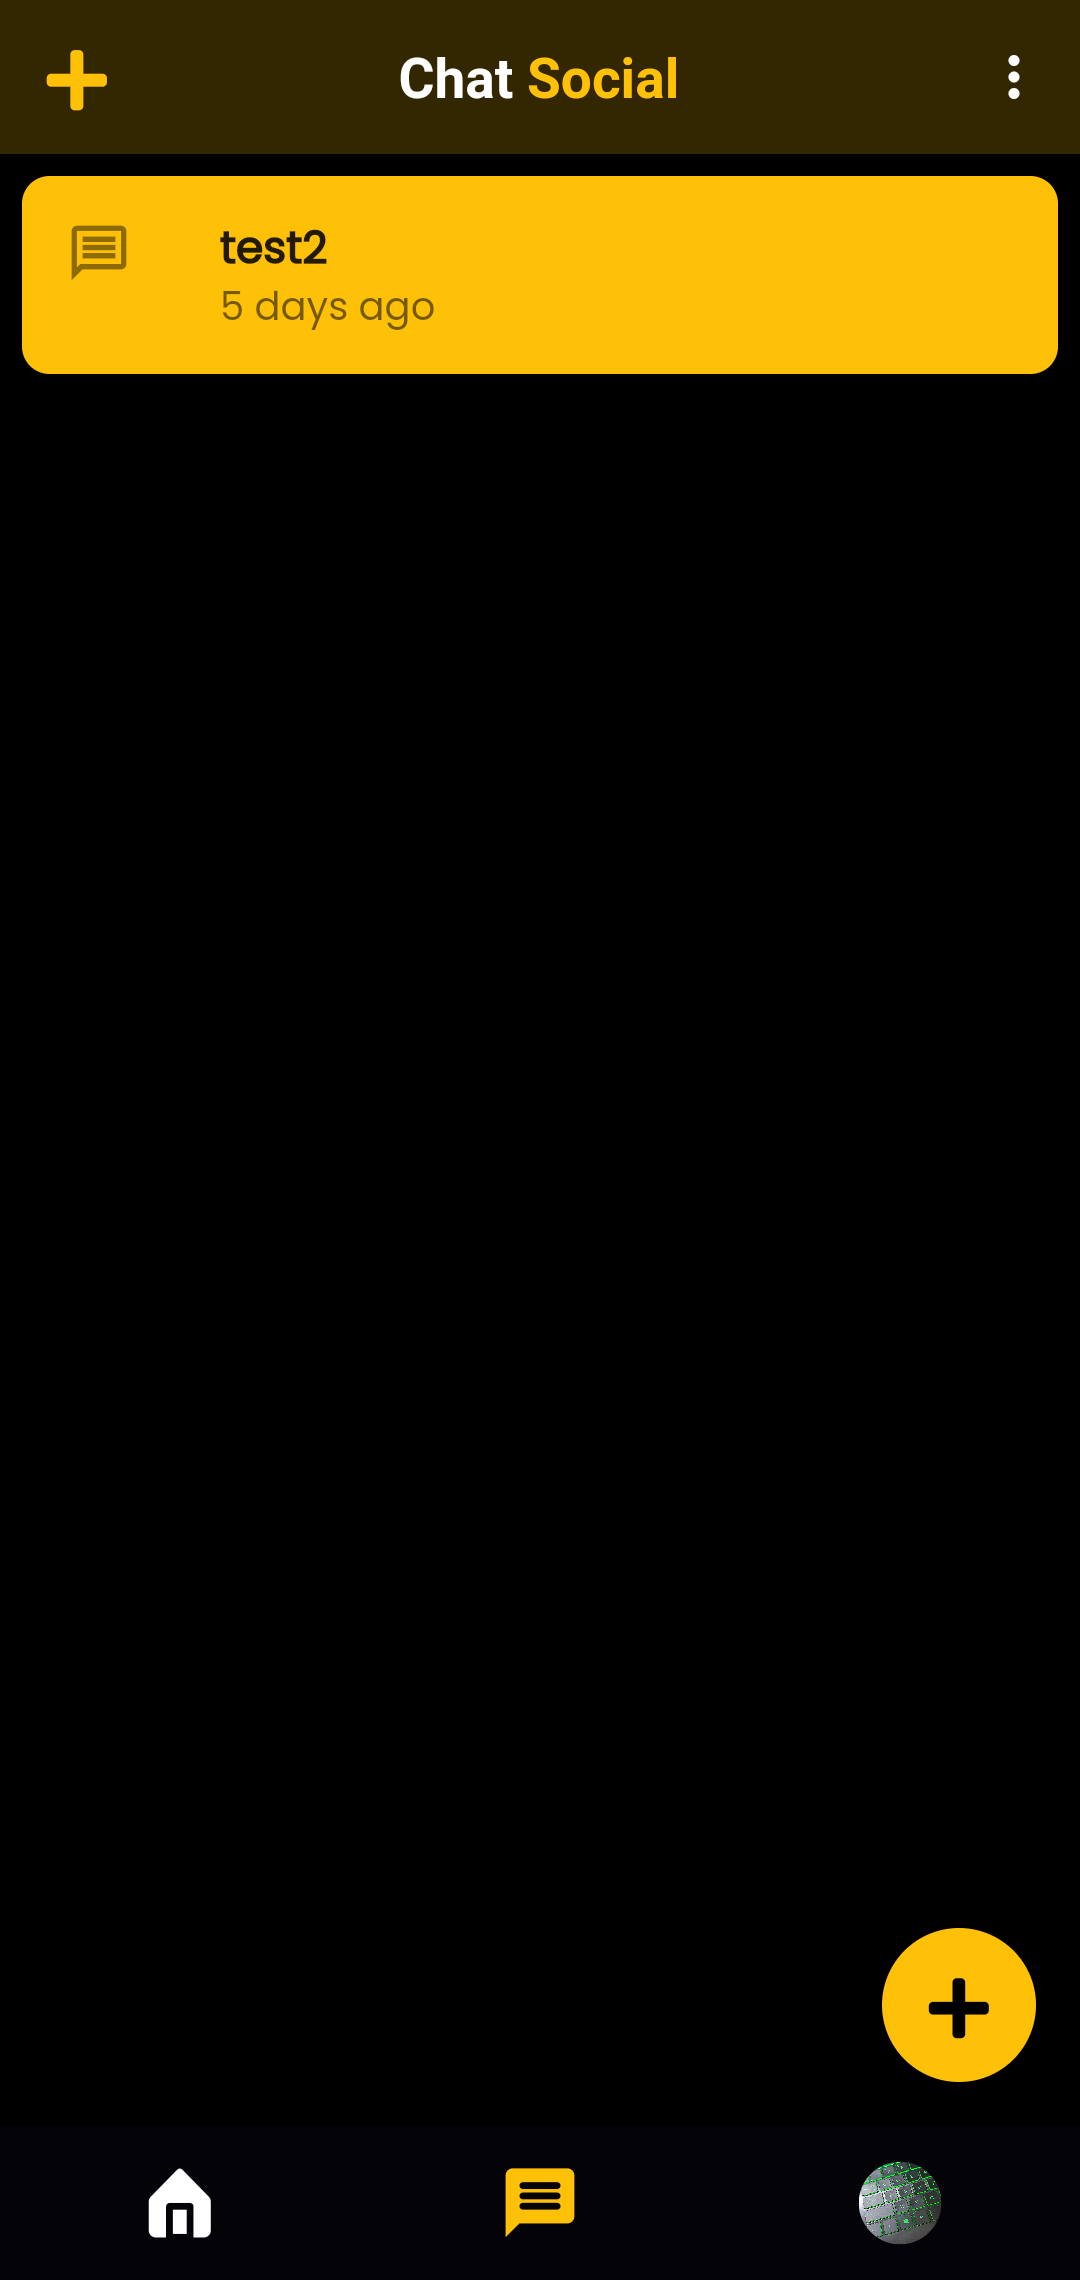
\includegraphics[scale=0.15]{App Screenshots/Group Chat screen.png}
    \caption{Group Chat Screen}
    \label{fig:Group Chat Screen}
\end{figure}

Then for sending messages in the chatroom we created a class called GroupMessage in "GroupMessage.dart" file and created a widget in that class for message screen with the title of chatroom name on the top header then we crated a scrollable view for all messages and at the bottom created a text field to type message and a send button beside it to send the message.

Now to handle the function to send the message we created another class called "GroupMessageHelper" and created a sendMessage method that creates a subcollection called "messages" under the document id in parent collection called "chatrooms" and adds the message along with its details such as timestamp and userid of the sender,his username and image.Then we call this method in the ontap function of the message send button using the provider.

To display the messages we created a method called "showMessages" in which we fetched the messages from the subcollection "messages" of chatrooms collection and displayed them in listview.

\begin{figure}[H]
    \centering
    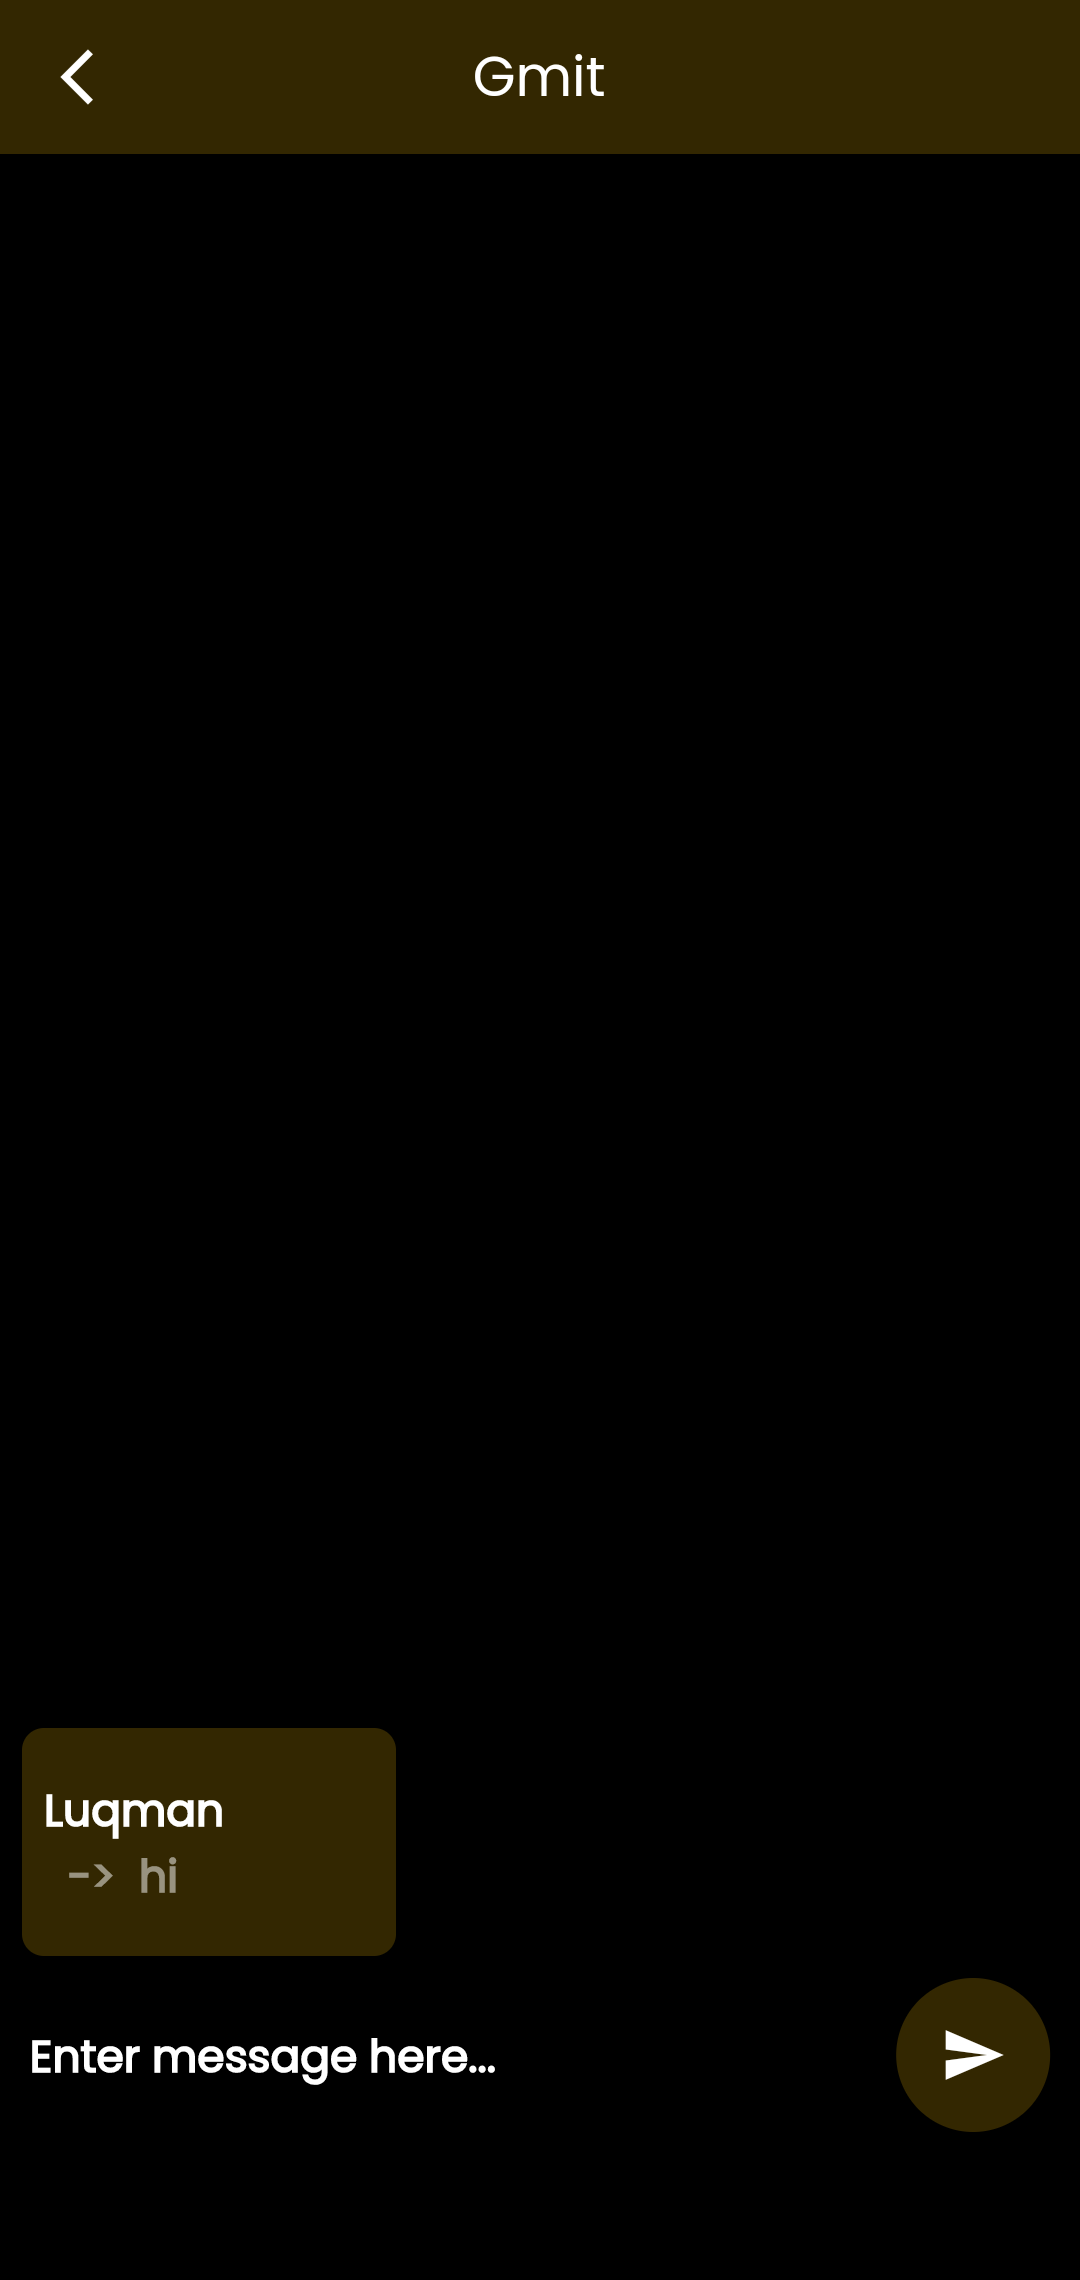
\includegraphics[scale=0.15]{App Screenshots/MessageScreen.png}
    \caption{Message Screen}
    \label{fig:Message Screen}
\end{figure}



\chapter{System Evaluation}
\section{Robust}
To make our app robust we followed the performance best practices mentioned in the flutter documentation that Accelerated the Development, Eliminated boilerplate code, and helped to build higher quality, robust app.
\subsection{Testing \& Performance}
We tested our app's robustness and performance using the Dart DevTools. it is a set of debugging and overall performance equipment for Dart and Flutter. These equipment are dispensed in IDEs such as VS Code in our case, the flutter tool, the web dev tool, and the dev tools package.
\subsection{Test Plan}
For testing our Application we did unit testing and system \& integeration testing along with development of the app and then after completion we Created a TestPlan First to test all the features so for that we created our test cases and logged them in an excel workbook as can been seen in \ref{fig:Test Plan ScreenShot 1}, \ref{fig:Test Plan ScreenShot 2}, \ref{fig:Test Plan ScreenShot 3}.

\begin{figure}[!htb]
    \centering
    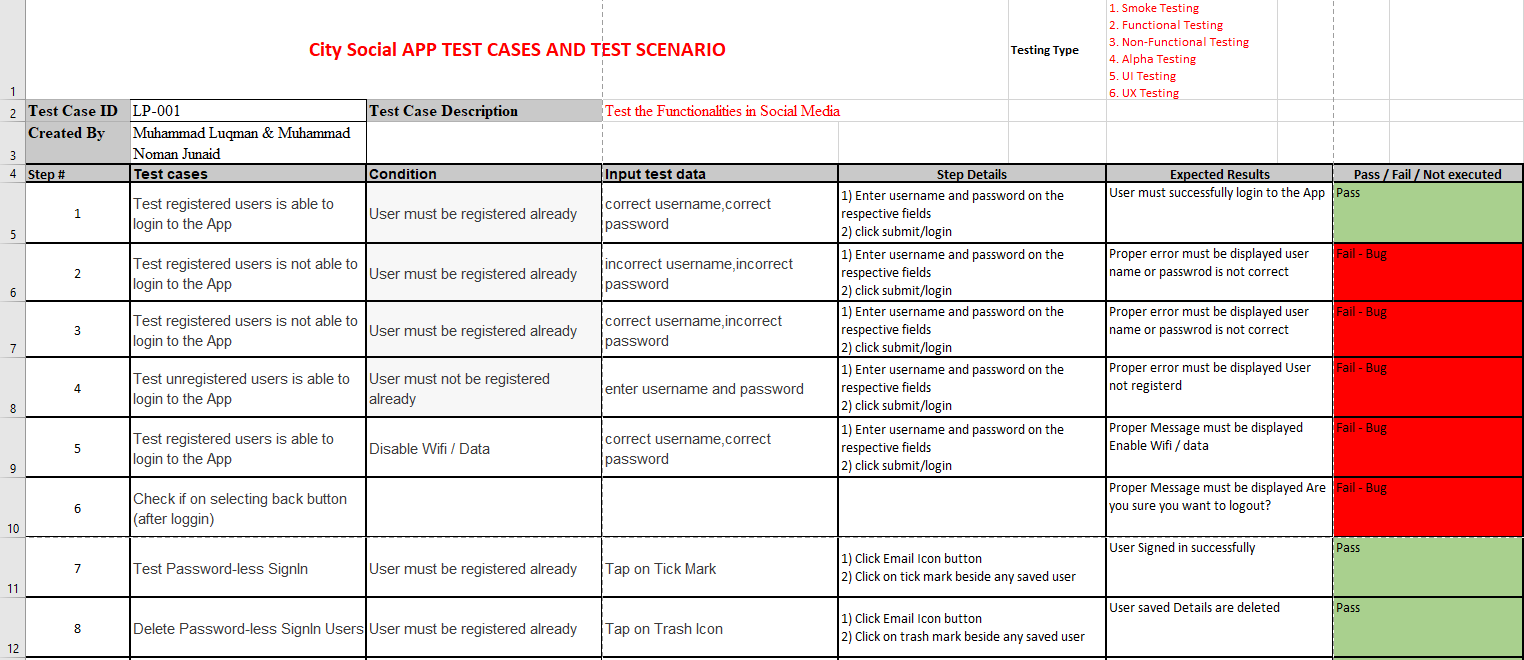
\includegraphics[scale=0.52]{testingshots/testplan1.PNG}
    \caption{Test Plan ScreenShot 1}
    \label{fig:Test Plan ScreenShot 1}
\end{figure}
\begin{figure}[!htb]
    \centering
    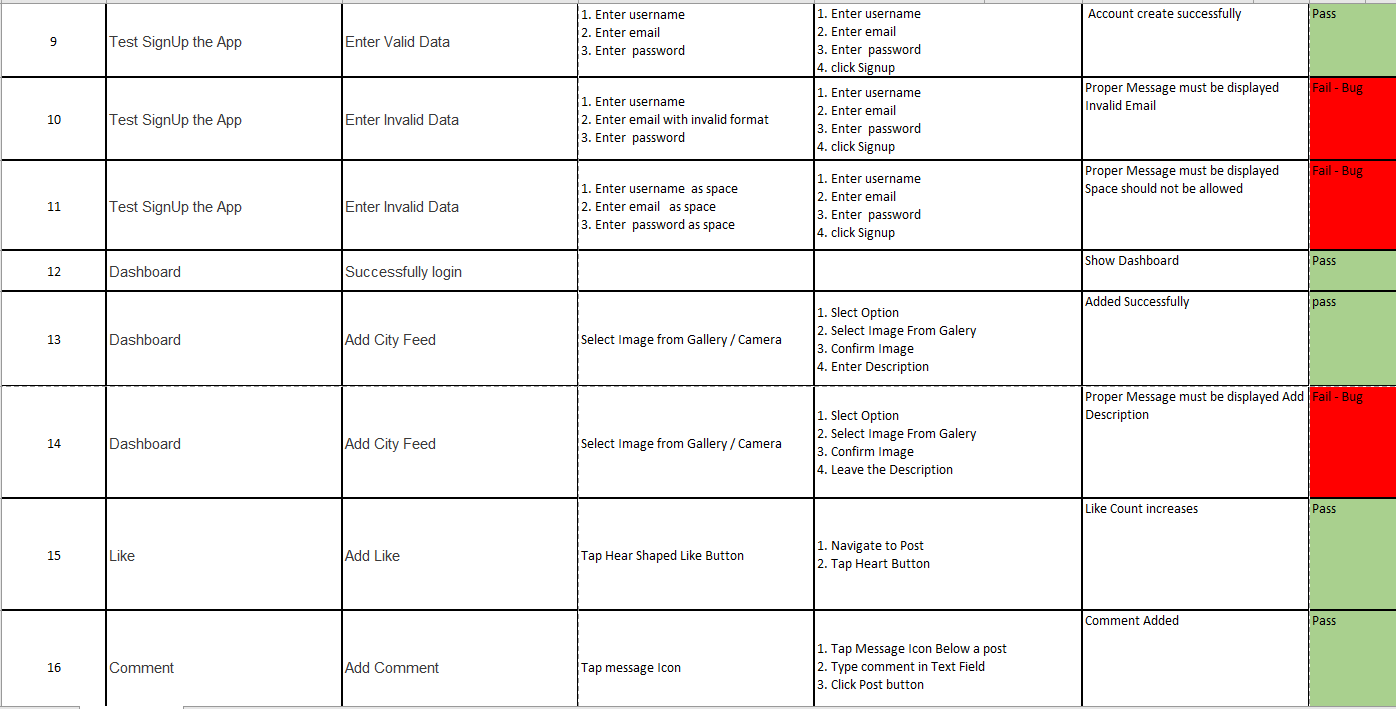
\includegraphics[scale=0.56]{testingshots/testplan2.PNG}
    \caption{Test Plan ScreenShot 2}
    \label{fig:Test Plan ScreenShot 2}
\end{figure}
\begin{figure}[!htb]
    \centering
    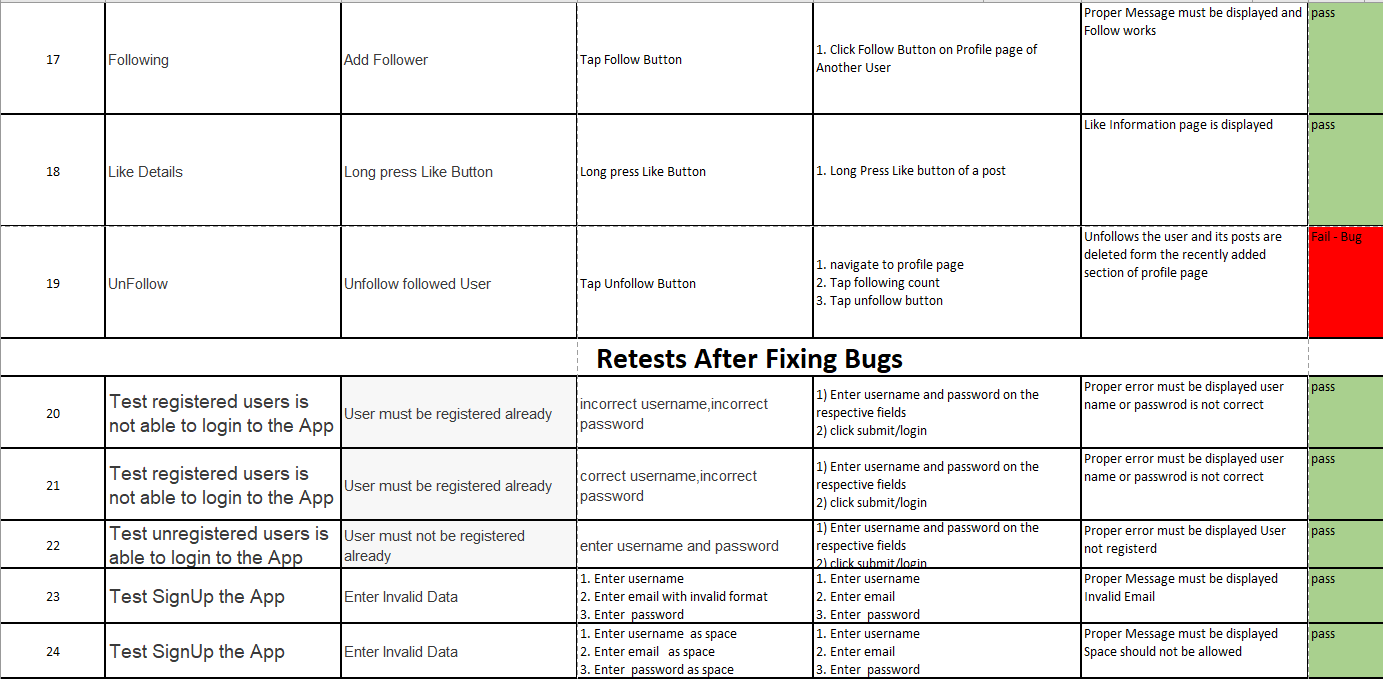
\includegraphics[scale=0.56]{testingshots/testplan3.PNG}
    \caption{Test Plan ScreenShot 3}
    \label{fig:Test Plan ScreenShot 3}
\end{figure}

After that we performed the Tests. The types of testing that we performed is below
\subsubsection{Unit Testing}
Every feature that was created, was tested first before integrating with the application testing was done by running the app on an emulator and then performing the operation on the developed feature and checking that does it perform the task that is expected or not. e.g saving posts to the firestore database after we press the post button, the post data should be saved to the firestore which was then verified by checking the database documents that does it contains the post data which was saved if yes that means it does what it is intended for so this passes the test.

\subsection{System Integration \& Testing}
The next stage or sprint was to focus on the integration of the features and their integration testing. First, we integrated the initial project structure with the firebase. Then we starting building app features, Unit testing them, and integrating them and testing them after integration like we developed the sign-in page and home page of the application then we unit tested them and then integrated and tested them after integration in a way that after the sign-in user is taken to the home page. so in this way we completed all the integration and testing.

\subsection{Smoke Testing}
Smoke Testing is a software program trying out process that assesses whether or not a software program construct is stable. It lets in the QA group to retain with the relaxation of the software program trying out. It is made of a small quantity of checks which might be run on every construct to affirm software functionality. "Build Verification Testing" or "Confidence Testing" are different phrases for smoke trying out.
\subsection{Functional Testing}
Functional Testing is a sort of software program checking out that validates the software program machine in opposition to the practical requirements/specifications. The motive of Functional checks is to check every characteristic of the software program application, with the aid of using imparting suitable input, verifying the output in opposition to the Functional requirements.It Can be done using automation tools or manually and we performed it manually.
\subsection{Non-Functional Testing}
Non-Functional Testing is described as a form of Software checking out to test non-practical aspects (performance, usability, reliability, etc) of a software program application. It is designed to check the readiness of a gadget as according to nonfunctional parameters which can be in no way addressed with the aid of using practical checking out.
\subsection{Alpha Testing}
Alpha trying out is the primary give up-to-give up trying out of a product to make certain it meets the enterprise necessities and capabilities correctly. It is commonly finished via way of means of inner personnel and performed in a lab/level environment. An alpha take a look at guarantees the product truly works and does the whole lot it’s prepurported to do.
\subsection{UI Testing}
UI Testing, additionally referred to as GUI Testing is essentially a method supposed to check the components of any software program that a person will come into touch with. This commonly method trying out the visible factors to affirm that they're functioning in line with requirements – in phrases of capability and performance. UI trying out guarantees that UI features are bug-free.
\subsection{UX Testing}
User experience testing is the process of evaluating various aspects of the user experience in order to discover the optimal method for a app and its components to interact with their visitors.
\subsection{Bugs \& Issues}
Following are the issues and Bugs found by the above testing techniques.
\begin{enumerate}
    \item \textbf{Login Panel Issue/Bug:} Enlisted Users are not being removed in some specific case.
    \item \textbf{Sign Up Issue/Bug:} New account should not be created if invalid email format is entered.
    \item \textbf{Sign Up Issue/Bug:} New account should not be created if User Name / Password field is empty.
    \item \textbf{Sign Up Issue/Bug:} The password field should display the characters in asterisks or bullets such that the password is not visible on the screen but it doesn't.
    \item \textbf{Login Issue/Bug:} There should be an alert “Invalid user name or password” or “User does not exist” if user enter invalid credential at signin page
    \item \textbf{Login Issue/Bug:} User should not login if the password field is empty
    \item \textbf{Back button Issue/Bug:} after logout pressing back button on welcome screen should not take the user back to profile page.
    \item \textbf{Keyboard on caption Issue/Bug:} Keyboard is opened on Add a caption field text box and hides it.
    \item \textbf{Chat screen back button Issue/Bug:} Application should not got to welcome screen while pressing back button from chat social screen.
    \item \textbf{Dashboard back button Issue/Bug:} user should be asked if user wants to logout while pressing back button form dashboard
\end{enumerate}
\subsubsection{Performance Test}
We started our app in profile mode. The Flutter profile mode builds and runs the application in a similar way to the release mode, but has enough advanced features to solve performance issues. To do this we just added a line of code``fluttermode:profile`` in the launch.json file of the project. Then we opened the dart dev tools and opened the performance tab of the dev tools and tested all the functionality of the app and recording the performance at the same time. 

Our app ran super smooth and responsive on the device that we deployed the app on which was "Samsung Galaxy S10". The average performance of the app was 60 FPS. As it is stated in flutter documentation \cite{PerformanceDocs:online} that ``If your frames are rendering in well under 16ms total in profile mode, you likely don’t have to worry about performance even if some performance pitfalls apply`` so considering this our overall app frame rendering was under 12ms so from this we can say that our app has no performance issues and Here is the screenshot for that below.

\begin{figure}[!htb]
    \centering
    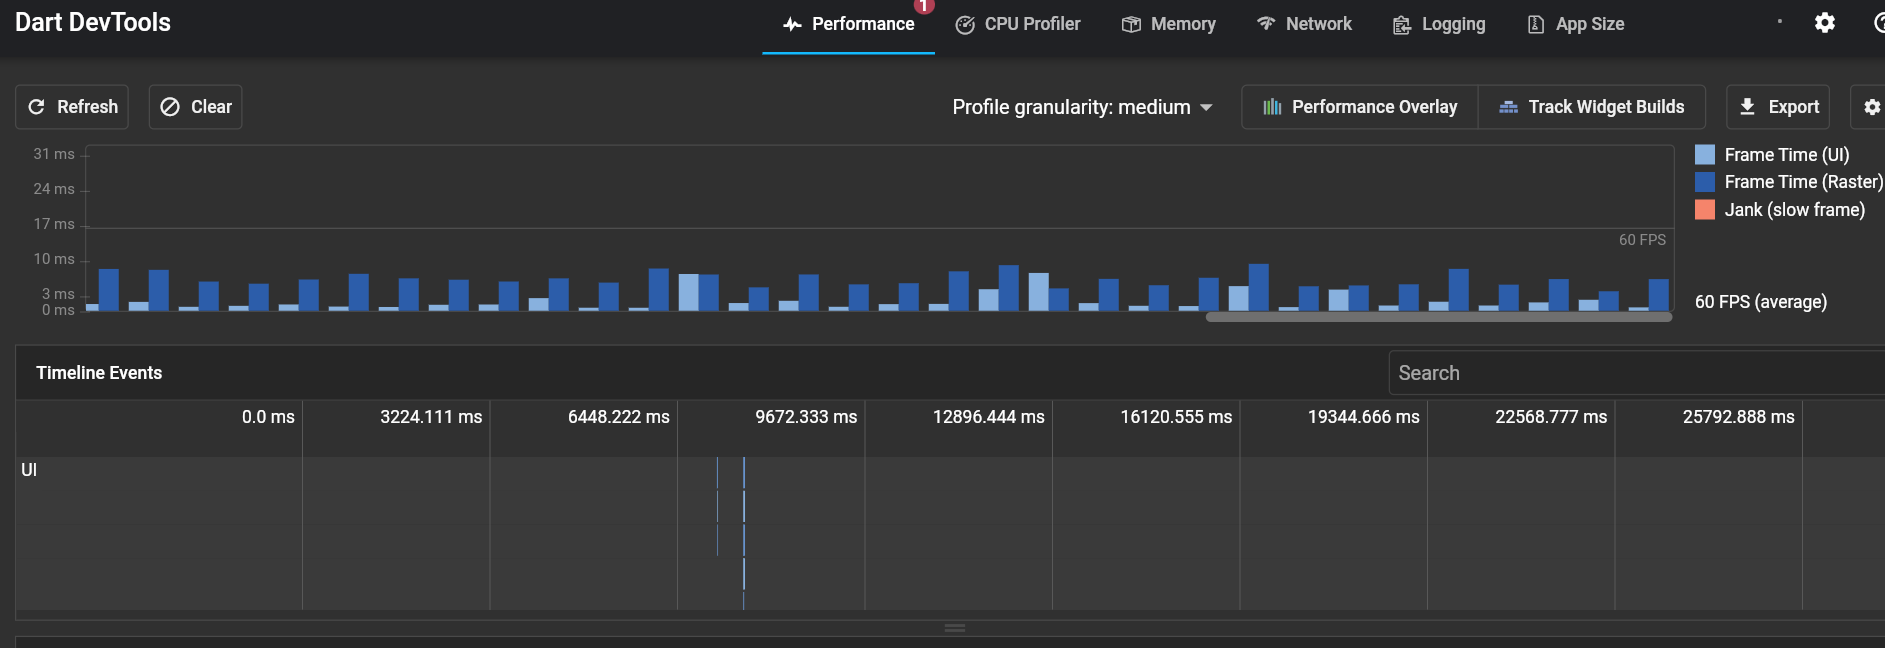
\includegraphics[scale=0.35]{img/performance test.PNG}
    \caption{Performance Test}
    \label{fig:Performance Test}
\end{figure}

\subsection{Performance Testing through Apptim}
We installed Apptim and connected our device "Samsung galaxy s10" through usb and started the test session then we mannualy test all the features of the app and tried to put pressure on the app by testing multiple features together.Below are the screenshots of the performance testing \ref{fig:Performance Test Summary}.

\begin{figure}[!htb]
    \centering
    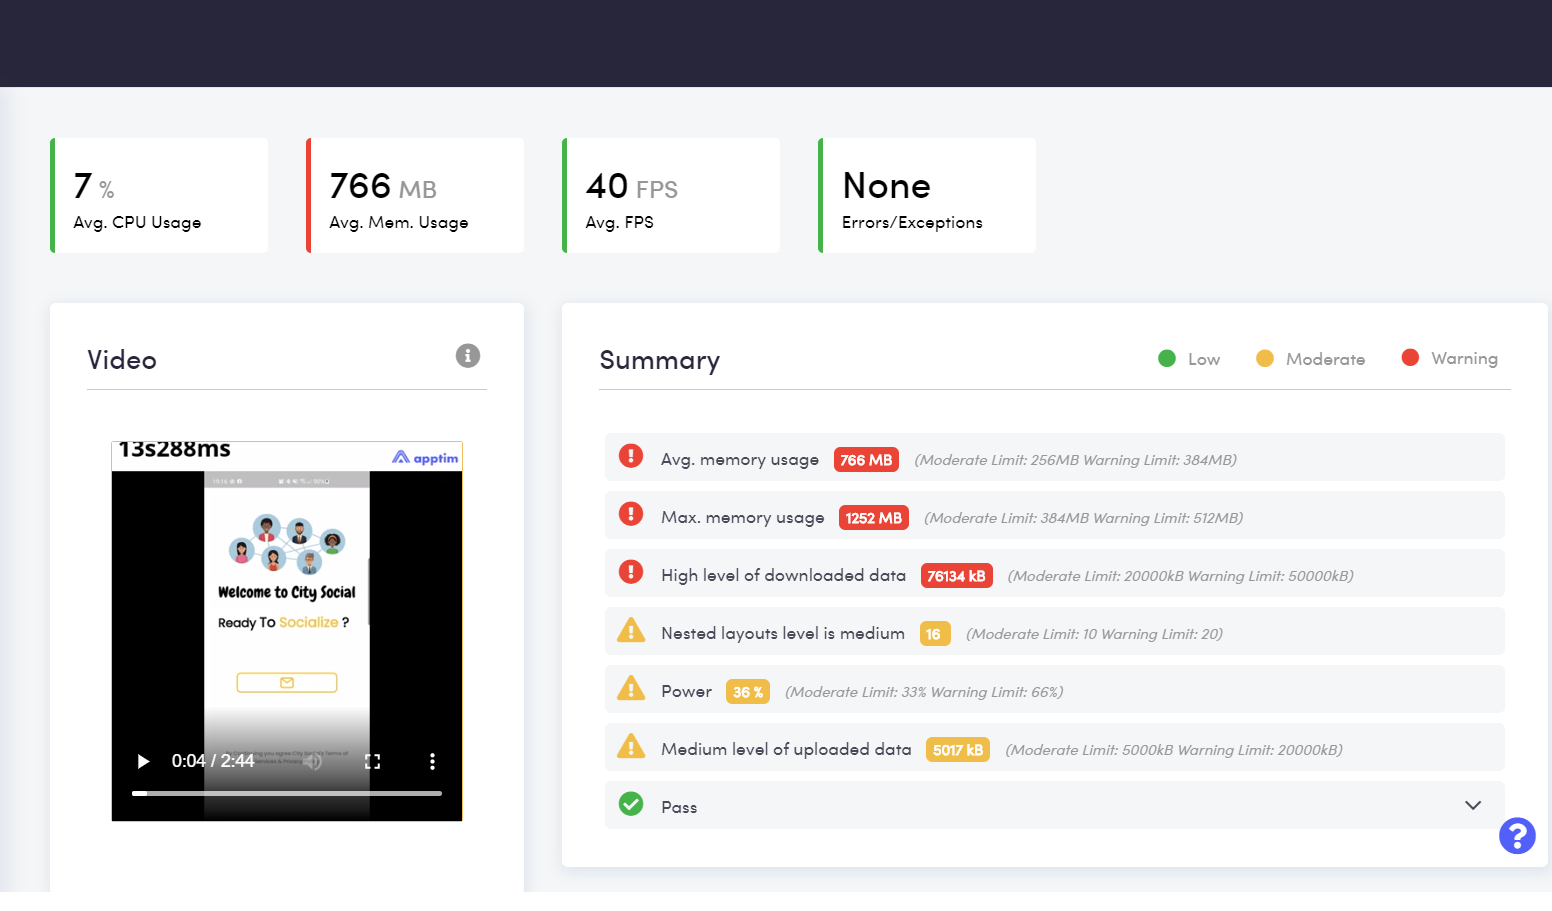
\includegraphics[scale=0.45]{testingshots/Performance1.PNG}
    \caption{Performance Test Summary}
    \label{fig:Performance Test Summary}
\end{figure}
On Average the Cpu usage was 7\% which seems pretty good. The memory usage was high but performance also depends on the device and 766mb usage should no be problem for devices of these days.The rendering rate was also good of 40 frames per second and power consumption was moderate and luckily there were no exceptions found.

We tested the app for about 5 minutes and again if testing is done for longer time we think results would be more accurate.The Screenshots of usage of resources are Below.

\begin{figure}[H]
    \centering
    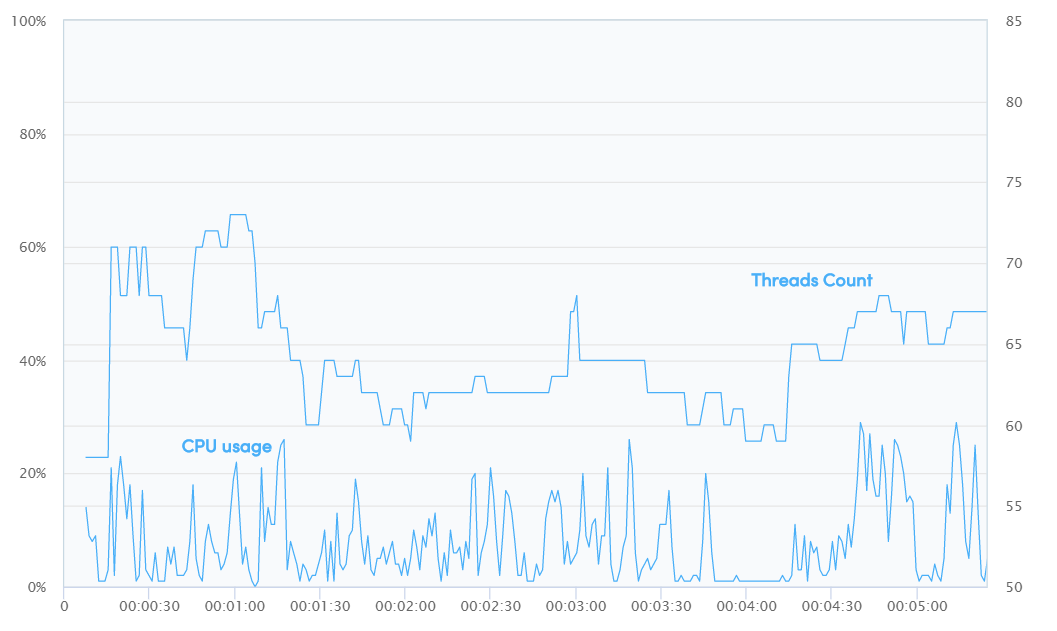
\includegraphics[scale=0.70]{testingshots/CpuUsage.PNG}
    \caption{Cpu Usage}
    \label{fig:Cpu Usage}
\end{figure}

\begin{figure}[H]
    \centering
    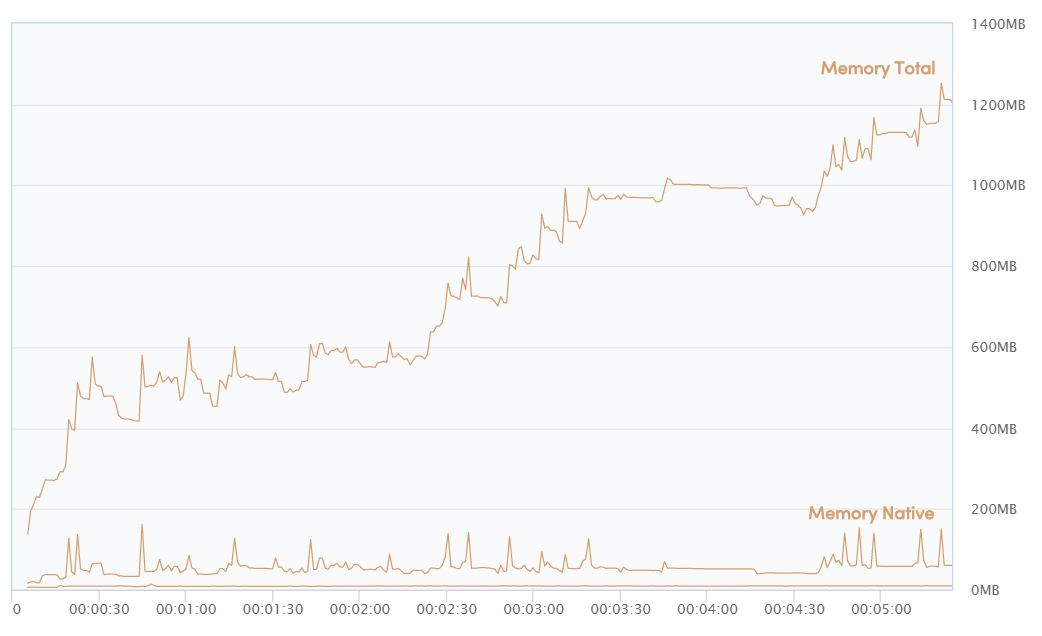
\includegraphics[scale=0.60]{testingshots/MemoryUsage.PNG}
    \caption{Memory Usage}
    \label{fig:Memory Usage}
\end{figure}

\begin{figure}[H]
    \centering
    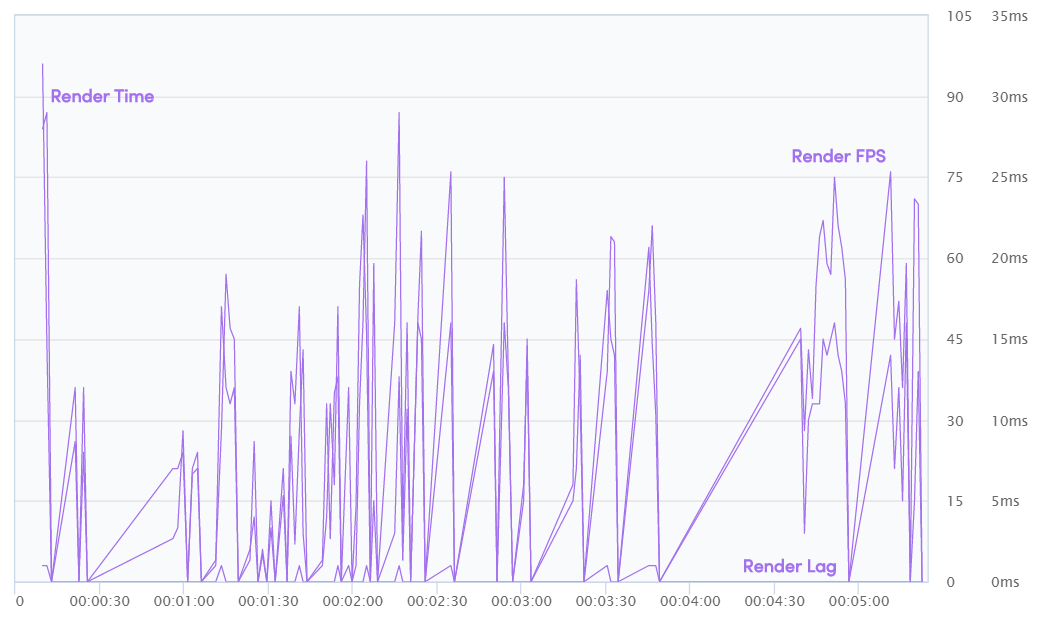
\includegraphics[scale=0.60]{testingshots/RenderTest.PNG}
    \caption{Render Test}
    \label{fig:Render Test}
\end{figure}

\begin{figure}[H]
    \centering
    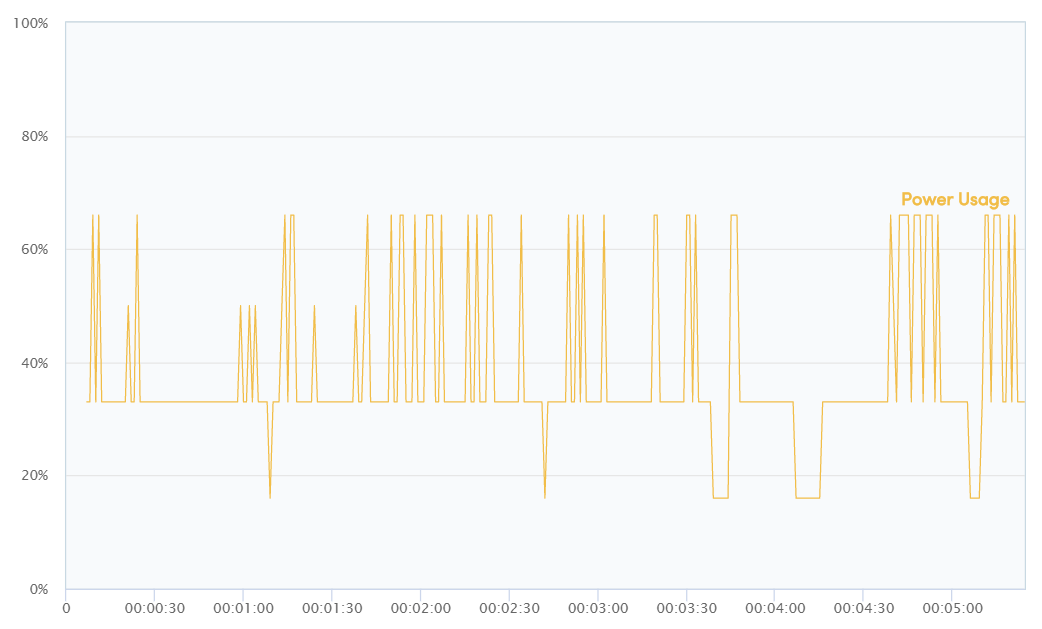
\includegraphics[scale=0.70]{testingshots/powerconsumption.PNG}
    \caption{Power Consumption}
    \label{fig:Power Consumption Test}
\end{figure}

\section{Evaluation of Objectives}
\subsection{Learning New Technology}
Our main goal for this project was to learn new technologies such as the Flutter framework, Dart programming language, and Firebase. As the career field that we choose is very competitive and continuously changing so for that reason to stay updated with the industry we have to learn new technologies. Through creating this project we have accomplished this goal.
\subsection{App Features}
Our goals for features were too high, although according to us we achieved around 75 to 80\% of what we wanted for this project as we couldn't implement some of the features such as Live Alerts and Push notifications, Activity Feed Notifications, Fingerprint Authentication, Publishing App to Play store, we will talk about them in detail in the limitations \& problems section. The features that we have successfully implemented are below.
\begin{itemize}
    \item Sign in Splash Page.
    \item Sign in using Email.
    \item Use of loading widgets.
    \item Upload post photo using camera or gallery.
    \item User profile.
    \item Display post count, followers count, and posts on the profile page.
    \item Like post.
    \item Realtime messaging with comments.
    \item Following or unfollowing user functionality.
\end{itemize}
\subsection{Scalable and Re-Usable}
The application scales very well and functions are set with Google's recommended
standards. The application is re-usable for any type of business and implementing a new feature is easy with how the application is set up.
\subsection{Responsiveness}
Our goal for the project to be responsive worked out well thanks to the development principles, Performance tips by the Flutter development team, and their great documentation that we followed. Not only is the Navigation very fast, but the read/also write from the database is almost instantaneous.

\section{Limitations and Problems we came across}
\subsection{Sign-Up Bug}
The first bug that we encountered was a sign up bug in which userid was not getting saved in the firestore making the inituser data asynchronous fixed the issue.
\subsection{Photo Upload Bug}
The second problem that we faced was that image was not uploading to the database so after debugging and printing the path where the image should be stored we found the path was incorrect so changing the path to correct one fixed the problem.
\subsection{Last timeline post Bug}
The last post of timeline feed was cutting off and not displaying properly so increasing the height of the container solved the issue.
\subsection{Bug in edit and delete post popup}
Bottom portion of edit and delete post was cutting off and not apearing properly
so we fixed that by decreasing the height of popup widget.
\subsection{Sign-in Bug}
if incorrect email and password was entered then user was still taken to the dashboard so fixed that by adding validation in the signin logic.
\subsection{Visible password bug}
The password field should display the entered characters in asterisks or bullets such that the password is not visible on the screen but it wasn't so we fixed it by using the obscuretext property and setting it to true.
\subsection{New Account with Empty Fields Bug}
New account could be created if User Name/ Email / Password field is empty so to fix that we used the form validation to have all these fields to be filled mandatory.
\subsection{Back Button Bugs}
There we Back button bugs in almost every screen such as tapping device's native back button would take the user from logged in state to log out without asking.From timeline page it took to welcome screen, from chat to login screen. 

so to fix that we defined the back button functionality in all screen to get rid of that unexpected behaviour / bug.
\subsection{keyboard on caption Bug}
keyboard of device opens on the Add a caption text box and hides it so to fix that we increased the height of the main widget which was containing all other child widgets.

\subsection{Unfollow Functionality}
we tried to implement the unfollow functionlity by using the logic that upon pressing the unfollow button the document related to that following id deletes from database but for some reason its not working so we will work on that in future.

\subsection{Publishing to play store}
As we couldn't implement all the required features as there is a saying that ``the first impression is the last impression`` so we decided not to publish the app until we have all the planned features implemented successfully and as we realized that if we publish the app and the app traffic increases and gets more requests it would cost us money on a monthly basis for using firebase.As free quota of firebase is 1Gb storage.

\subsection{Ios limitation}
We couldn't Test the app for ios as for Ios we need Xcode for it which is not supported on windows and it required a mac for that and neither of us owns a mac and we thought it would not be feasible to buy or rent a mac for Ios implementation.

\chapter{Conclusion}

This part of our dissertation will review our project in terms of the purpose of the original intentions and examine our findings and the result of the project when we had completed it. Hopefully, by the end of reading this chapter, the reader will gain an insight into how both of us feel about the project and what we learned during the development.

\section{Context Summary}
Our final year project was the development of a Flutter Application build using Visual Studio Code, Firebase, Flutter \& Dart which was a photo-sharing social media application on which a person can socialize with other people and friends who also use this application. It has various features but the most important ones are sharing images in form of posts with caption, liking and commenting on the posts of others users. Following other users, having a profile with photos, name, Counts and group chatting.
\section{Objectives Conclusion}
We have achieved our objectives such as learning new technologies. Although we went through the documentation of them and now have basic to intermediate knowledge about these technologies but we still need to read complete documentation of these technologies as we only used some part of these techs and to reach the advanced level of programming with these technologies we need more practice as there are famous sayings that ``practice make a man perfect and Rome was not built in a day``

we achieved another object by making the app scalable and re-usable and in Future we have planned to add more features to it. In terms of responsiveness which was another object that we carried off successfully by making a responsive app but as we say there is always room for improvement so we will work on our further to make it more responsive.

In terms of feature implementation which was another objective we were able to implement about 75 to 80\% of the features that we planned and the rest that we mentioned above that we couldn't get working, so we intend to work on them in future.

\section{opportunities identified}
we think that there is a lot of scope in expanding the application and many more features can be implemented to make the app more intuitive.
\subsection{status feature}
These days this feature is the most used one as we are social networking user our selves and everyone is using this feature every day. Basically, it displays a post (image or video) for 24 hours and the owner can also identify who saw their status. it's something similar to news headlines.
\subsection{video posts feature}
Video posing is also a very important feature these days it is similar to image posts that we have implemented but it's a video instead of images.
\subsection{Direct message (DM)}
This is a chat feature in which there is an inbox where all messages are stored and users can chat with other users who are following each other.
\subsection{Live Broadcasting}
This feature is also very popular these days due to the covid-19 pandemic. It's a kind of a video call feature but instead of one to one the video and voice is broadcasted to all followers and they all can view it and comment on it or can request to join the user that is broadcasting.

\section{Final reflections of the Project}
\begin{itemize}
    \item Using Scrum Agile Methodology helped maintain a good architecture to our development progress. We found that having a weekly meeting with our supervisor assigned to us Dr.Dominic Carr helped us keep on track on the development of the project and provided feedback on weekly meetings. We also then had our one-to-one Team meetings with each other every Monday to see how we're getting on and to see if we can fix any errors we had before our meeting every week on Wednesdays with our supervisor. However, there were still a few setbacks in these meetings as internet connection varied for some and technical issues happened at times. None the less we still were able to talk to one another at times. The Scrum Agile Methodology had been hugely helpful for us and was easy to follow.
    \item Overall the whole development of our final year project was indeed at times challenging but at the same time a worthwhile experience. Even though we both did not achieve everything we had set out at the beginning of the development as there were many aspects that were challenging as sometimes we sometimes were unable to find certain resources at time and then the lockdown being in place which limited us from working together on the project. However, still, we both attained a good insight in using Flutter while coding and insight into various technologies we used in the project. We also obtained a better bond giving each other support through the various endeavors and issues, while at the same time maintaining a positive attitude throughout the project's development even with a worldwide pandemic happening at the same time. In the end of all this with all the research, effort, and development that was put into our joint final year project, we were both happy with the end product of the project and we both were proud of ourselves as we now know it feels to work on small scale project now and will be able to work on any other future small scale projects we may have to develop in the future and we now both feel more confident as software developers now.
\end{itemize}

\chapter{Appendices}
\section{GitHub Repository}
\url{https://github.com/LuqmanFarooq/Final-Year-Project-And-Dissertation}

\section{Github Kanban Board}
\url{https://github.com/LuqmanFarooq/Final-Year-Project-And-Dissertation/projects?query=is%3Aclosed}


\section{Installation Instructions}
\begin{enumerate}
    \item Navigate to the Repository and then to the ``2-APK FILE`` folder in root.
    \item Download the release-apk file.
    \item copy it to any android phone.
    \item install the apk and give permission to trust app installation from unknown sources.
    \item Open and use the App.
\end{enumerate}
\printbibliography